\documentclass[11pt,a4paper]{article}

% -------------------------------------------------
% Packages
% -------------------------------------------------
\usepackage[utf8]{inputenc}
\usepackage[T1]{fontenc}
\usepackage{lmodern}
\usepackage{tikz}
\usepackage{geometry}
\geometry{margin=1in}

\usepackage{amsmath, amssymb, amsfonts}
\usepackage{bm}

\usepackage{graphicx}
\usepackage{float}
\usepackage{caption}
\usepackage{subcaption}

\usepackage{booktabs}
\usepackage{multirow}

\usepackage{hyperref}
\hypersetup{
    colorlinks=true,
    linkcolor=blue,
    citecolor=blue,
    urlcolor=blue
}

\usepackage{natbib}
\usepackage{doi}

\usepackage{setspace}
\onehalfspacing

% -------------------------------------------------
% Custom commands
% -------------------------------------------------
\newcommand{\GW}{gravitational-wave}
\newcommand{\GWs}{gravitational waves}
\newcommand{\LIGO}{LIGO}
\newcommand{\Virgo}{Virgo}

% -------------------------------------------------
% Title information
% -------------------------------------------------
\title{\textbf{Template-Free Geometric Analysis of Gravitational-Wave Events}}

\author{
Marcelo Burgos\\
\small Independent Researcher\\
\small \texttt{mburgos@hackfluency.com}
}

\date{\today}

% -------------------------------------------------
\begin{document}
\sloppy
\emergencystretch=1em
% -------------------------------------------------

\maketitle

\begin{abstract}

We present a novel geometric analysis of gravitational-wave signals based on the structure of whitened strain data from interferometric detector networks. While whitening is a standard preprocessing step in gravitational-wave data analysis, we reinterpret the resulting strain space as a geometric arena in which coherent spacetime deformations induced by gravitational waves manifest as dominant, low-dimensional modes. By constructing spectral operators from band-limited, time-localized whitened data, we identify robust geometric modes that remain invariant across frequency sub-bands, temporal subsegments, and detector configurations. We demonstrate that these modes can be consistently compared across different gravitational-wave events without the use of waveform templates, enabling a new, model-independent classification scheme. Our results suggest that gravitational-wave events possess an internal geometric structure that is directly observable in current interferometers and may encode fundamental information about the underlying spacetime dynamics.

\end{abstract}

\section{Introduction}

The direct detection of gravitational waves (GWs) by the LIGO and Virgo collaborations has opened a new observational window into the Universe, enabling the study of compact-object mergers and strong-field gravity \cite{Abbott2016, Bailes2021}. Current gravitational-wave data analysis pipelines rely predominantly on matched filtering techniques \cite{Creighton2011, Usman2016}, where detector data are compared against large banks of theoretical waveform templates derived from General Relativity. While this approach has proven extraordinarily successful for detection and parameter estimation, it inherently presupposes a model for the signal morphology and source dynamics.

In parallel, unmodeled or weakly modeled searches, such as burst analyses, aim to identify coherent excess power across detector networks without relying on detailed waveform templates \cite{Klimenko2016, Sutton2010, Abbott2021BurstO3}. These methods focus primarily on detection significance rather than on uncovering internal structural properties of the signal itself.

In this work, we adopt a complementary perspective. Rather than optimizing detection or parameter recovery, we investigate the \emph{geometric structure} of gravitational-wave signals as manifested in the detector network. Specifically, we demonstrate that gravitational-wave events induce robust, coherent geometric modes in the whitened strain space of interferometric detectors, revealing an internal structure that is remarkably stable across frequency bands, temporal subsegments, and detector combinations.

Concretely, the analysis proceeds by whitening each detector time series (thereby defining the noise-weighted metric), restricting to a chosen frequency band, and constructing short-time Fourier transforms (STFTs) over overlapping windows.
We then identify a data-driven set of \emph{active} windows (high combined narrowband energy across detectors), build a stacked detector$\otimes$frequency network representation, and form a network spectral operator whose eigenstructure defines the coherent geometric modes.
For classification we further suppress empirically estimated instrumental subspaces using an off-source projector, yielding a projected operator from which scalar observables (e.g., $\eta_{\mathrm{proj}}$ and eigenvalue ratios) are computed \cite{Acernese2023VirgoDetCharTools}.
For the wavefront reconstruction case study, we organize the geometry into three fixed bands used throughout: inspiral $[30,80]$~Hz, post-inspiral $[80,150]$~Hz, and merger-ringdown $[150,300]$~Hz.

Throughout, the primary spectral operators (and their eigenmodes) live in the stacked detector$\otimes$frequency space, while detector-only quantities (e.g., three-component participation vectors or $\mathbf{C}_{\mathrm{det}}$ plots) are explicitly defined reductions used for interpretability.
By “template-free” or “model-independent” we mean that no waveform templates or source priors are used; the method still assumes standard preprocessing choices such as whitening/PSD estimation, band selection, and windowing \cite{Creighton2011, Usman2016, Acernese2023VirgoDetCharTools}.

\subsection{Whitened strain as a geometric space}
\label{sec:whitened_strain_space}

Gravitational-wave interferometers measure the dimensionless strain time series $h(t)$, which is contaminated by colored, non-stationary noise and transient instrumental artifacts \cite{Acernese2023VirgoDetCharTools, Tolley2023ArchEnemy}. A standard preprocessing step in gravitational-wave data analysis is \emph{whitening}, which transforms the data into a space where the noise has (approximately) unit variance and is uncorrelated across frequencies.

Let $\tilde{h}(f)$ denote the Fourier transform of the strain signal, and let $S_n(f)$ be the one-sided noise power spectral density (PSD) of the detector. The whitened strain $\tilde{h}_w(f)$ is defined as
\begin{equation}
\tilde{h}_w(f) = \frac{\tilde{h}(f)}{\sqrt{S_n(f)}}.
\end{equation}
Transforming back to the time domain yields the whitened time series $h_w(t)$.

This transformation induces a natural inner product between two strain signals $a(t)$ and $b(t)$,
\begin{equation}
\langle a, b \rangle = 4 \, \mathrm{Re} \int_0^\infty \frac{\tilde{a}(f)\tilde{b}^*(f)}{S_n(f)} \, df,
\end{equation}
which is ubiquitous in gravitational-wave data analysis \cite{Creighton2011}. In this metric, stationary Gaussian noise becomes isotropic, and physically coherent signals are geometrically emphasized.

While whitening is routinely employed as a preprocessing step, it is typically regarded as a technical normalization enabling optimal filtering. In contrast, we interpret the whitened strain space as a \emph{geometric arena} in which gravitational-wave signals manifest as structured, low-dimensional coherent modes.

\subsection{Geometric modes and network coherence}

By constructing spectral operators from the whitened, band-limited strain data across multiple detectors, we identify dominant eigenmodes corresponding to coherent geometric deformations induced by gravitational waves. These modes exhibit strong invariance properties under:
\begin{itemize}
\item frequency sub-band selection,
\item temporal subsampling within the event,
\item projection against instrument-dominated subspaces,
\item and detector-network reconfigurations.
\end{itemize}

Importantly, these geometric modes can be directly compared across different astrophysical events, enabling a template-free classification scheme based solely on their internal structure. Our analysis reveals that events with distinct astrophysical properties may nevertheless share highly similar geometric modes, suggesting a deeper organizing principle in the detector response to spacetime perturbations.

\subsection{Scope and significance}

The objective of this paper is not to replace existing detection or parameter-estimation pipelines, but to introduce a new framework for analyzing gravitational-wave data: one that focuses on the intrinsic geometric organization of the signal as observed by interferometric networks. This approach provides a novel, model-independent perspective on gravitational-wave events and opens the door to new classification strategies, consistency tests, and potential connections to fundamental aspects of spacetime dynamics.

\subsection{Relation to standard time--frequency representations}

Gravitational-wave events are commonly visualized using time--frequency spectrograms of the whitened strain for each detector individually. These representations, routinely published by the LIGO and Virgo collaborations, display the normalized spectral energy as a function of time and frequency, typically spanning several hundred Hertz and a time window of order one second around the event.

Such spectrograms are obtained by computing a short-time Fourier transform (STFT) of the whitened strain,
\begin{equation}
P_d(t,f) = |\mathrm{STFT}[h_{w,d}(t)]|^2,
\end{equation}
where $d \in \{\mathrm{H1}, \mathrm{L1}, \mathrm{V1}\}$ labels the detector. The resulting power is often normalized relative to off-source noise to enhance visual contrast. These plots provide an intuitive depiction of the chirp-like frequency evolution characteristic of compact binary coalescences and serve as an important validation and diagnostic tool.

Standard spectrograms treat each detector independently and encode information primarily through local energy density in the time--frequency plane. They do not explicitly capture the joint geometric structure of the detector network, nor are they designed to reveal invariant or low-dimensional patterns shared across detectors or across different events.

The approach presented here uses the same fundamental ingredients—whitened strain, band-limited STFTs, and time localization—but combines them into spectral operators defined on the multi-detector data space. Rather than analyzing energy distributions, we study the dominant eigenmodes of these operators, which represent coherent geometric structures induced by gravitational-wave signals. This mode-based geometric analysis enables direct comparison between events and reveals internal structures that are not apparent in standard time--frequency representations.

\subsection{From detector-level representations to coherent geometric modes}

Gravitational-wave observations are traditionally presented and analyzed at the level of individual detector responses. For a given event, each interferometer records a time--frequency representation of the strain data, typically shown as spectrograms spanning a broad frequency range and a narrow temporal window around the merger time. These representations emphasize the local response of each detector to the passing gravitational wave and constitute the standard visualization used by the LIGO--Virgo Collaboration.

As an illustrative example, Fig.~\ref{fig:gw170814_comparison}a shows the official detector-level spectrograms for the event GW170814, as published by the LIGO--Virgo Collaboration \cite{Abbott2017GW170814}. Each panel corresponds to a different interferometer (H1, L1, and V1), displaying normalized energy in the time--frequency plane. While these plots clearly reveal the presence of a coherent astrophysical signal across the network, they treat each detector independently and do not explicitly encode the joint geometric structure of the response.

In contrast, the approach developed in this work shifts the focus from detector-level representations to the identification of coherent geometric structures emerging from the network as a whole. Working in the standard whitened strain space, we construct spectral operators whose dominant eigenmodes capture the intrinsic geometry of the detector responses during the event. These modes are not reconstructions of the strain time series, nor template-based waveform estimates, but rather eigenstructures characterizing the collective deformation pattern induced by the gravitational wave across the interferometer network.

Figure~\ref{fig:gw170814_comparison}b presents the dominant geometric mode extracted for GW170814 using our method. This mode summarizes the relative participation and phase structure of the detectors within a single coherent object, providing a compact and physically meaningful representation of the event. As shown throughout this work, such geometric modes exhibit remarkable stability under variations in time, frequency band, and instrumental subspace projections, and enable direct comparisons between different gravitational-wave events without reliance on waveform templates.

Together, these representations highlight the conceptual transition underlying this study: from individual detector spectrograms to network-level geometric modes, opening a new pathway for the analysis and classification of gravitational-wave signals.

\section{Related Work}
\label{sec:related}

The framework developed here uses standard ingredients from gravitational-wave data analysis while introducing a distinct, operator-based focus on network-level coherence structure.

\paragraph{Whitening and matched filtering.}
Whitening is a standard preprocessing step that renders noise approximately white and stationary, enabling optimal matched filtering \cite{Creighton2011, Gabbard2018}. The inner product induced by whitening is central to gravitational-wave detection and parameter estimation. While we use the same mathematical foundation, we reinterpret whitened strain as a geometric space in which signals manifest as low-dimensional coherent modes, rather than as a technical step toward template matching.

\paragraph{Unmodeled burst searches.}
Burst searches seek coherent excess power across detector networks without assuming specific waveform morphology \cite{Klimenko2016, Sutton2010, Abbott2021BurstO3}. Methods like the coherent WaveBurst (cWB) algorithm construct network statistics that capture coherent energy but are primarily designed for detection, not for extracting geometric structure. In this paper we focus on the eigenstructure of the network spectral operator, which reveals invariant geometric modes that persist across frequency and time.

\paragraph{Principal component analysis in gravitational-wave data.}
PCA and related dimensionality-reduction techniques have been applied to gravitational-wave data for noise subtraction and glitch classification \cite{Cornish2015, Powell2021, Tolley2023ArchEnemy}. However, these applications typically treat single-detector data or focus on noise characterization. Our approach applies eigen-decomposition to the multi-detector network operator constructed from whitened strain, aiming to uncover geometric properties of the astrophysical signal itself.

\paragraph{Network null streams and consistency tests.}
Null-stream constructions \cite{Wen2008, Chatziioannou2019} use linear combinations of detector data to cancel gravitational-wave signals, providing a tool for noise characterization and signal validation. Our projection against instrumental subspaces shares a similar mathematical motivation but is used here to isolate astrophysical coherence for geometric analysis rather than to cancel signals.

\paragraph{Geometric approaches in other fields.}
The idea of analyzing signals through the geometry of their representation space has appeared in other domains, such as manifold learning for audio or image processing \cite{Roweis2000}. To our knowledge, this is the first application of such geometric reasoning to gravitational-wave network data for classification and wavefront reconstruction.

Overall, the method combines whitening, multi-detector coherence, eigen-analysis, and geometric interpretation into a unified framework for gravitational-wave characterization.

\section{Construction of Coherent Geometric Modes}
\label{sec:construction}

In this section we describe the mathematical framework used to extract coherent geometric modes from gravitational-wave data. Starting from the whitened strain measured by an interferometric detector network, we construct network-level spectral operators whose dominant eigenmodes encode the intrinsic geometric structure induced by a passing gravitational wave. We then discuss how these modes can be interpreted, reconstructed, and tested for physical robustness.

\subsection{Multi-detector whitened strain representation}

Consider a network of $N_d$ interferometric detectors indexed by $d \in \{1,\dots,N_d\}$.
For each detector, we work with the whitened strain time series $h_{w,d}(t)$, as defined in Section~\ref{sec:whitened_strain_space}.

We restrict the analysis to a finite time interval $[t_0, t_1]$ surrounding the event and to a frequency band $[f_{\min}, f_{\max}]$ of interest.
The whitened strain is decomposed using a short-time Fourier transform (STFT),
\begin{equation}
X_d(t_k, f_\ell) = \mathrm{STFT}\!\left[h_{w,d}(t)\right],
\end{equation}
where $\{t_k\}$ denote discrete time windows and $\{f_\ell\}$ denote frequency bins within the selected band.

For convenience we collect these coefficients into a band-limited STFT matrix for each detector,
\begin{equation}
\mathbf{Z}_d \in \mathbb{C}^{N_f \times N_t},
\qquad
[\mathbf{Z}_d]_{\ell k} = X_d(t_k,f_\ell),
\end{equation}
where $N_f$ is the number of frequency bins in the band and $N_t$ is the number of time windows.

For each time--frequency tile $(t_k, f_\ell)$, we collect the detector responses into a complex-valued network vector
\begin{equation}
\mathbf{x}(t_k, f_\ell) =
\begin{pmatrix}
X_1(t_k, f_\ell) \\
X_2(t_k, f_\ell) \\
\vdots \\
X_{N_d}(t_k, f_\ell)
\end{pmatrix}
\in \mathbb{C}^{N_d}.
\end{equation}

This vector represents the instantaneous network response to spacetime perturbations at a given time and frequency, expressed in a common, noise-normalized geometric space.

\subsection{Time--frequency aggregation and spectral operator}

To extract coherent structure, we first identify a subset of \emph{active} time windows
$\mathcal{T}_{\mathrm{active}} \subset \{t_k\}$ associated with the event using a robust, data-driven criterion
(e.g.\ percentile thresholding of combined band-limited energy across detectors).
Within a chosen band, we then form a network-embedded, stacked time--frequency vector at each active window by concatenating frequency bins across detectors,
\begin{equation}
\mathbf{z}(t_k)
=
\begin{pmatrix}
\mathbf{Z}_1(:,k) \\
\mathbf{Z}_2(:,k) \\
\vdots \\
\mathbf{Z}_{N_d}(:,k)
\end{pmatrix}
\in \mathbb{C}^{N_d N_f},
\end{equation}
where $\mathbf{Z}_d(:,k)\in\mathbb{C}^{N_f}$ denotes the column of STFT coefficients at time window $t_k$.

The corresponding \emph{network spectral operator} (the object used in the pipeline) is
\begin{equation}
\mathbf{C}_{\mathrm{net}}
= \frac{1}{|\mathcal{T}_{\mathrm{active}}|}
\sum_{t_k\in\mathcal{T}_{\mathrm{active}}}
\mathbf{z}(t_k)\,\mathbf{z}^\dagger(t_k)
\in \mathbb{C}^{(N_d N_f)\times(N_d N_f)}.
\end{equation}
This operator is Hermitian and positive semidefinite, and it captures second-order correlations in the full (detector $\otimes$ frequency) network space.

For physical interpretation focused purely on detector participation, it is also useful to define a reduced detector-space operator obtained by averaging over frequency bins,
\begin{equation}
\mathbf{C}_{\mathrm{det}}
= \frac{1}{|\mathcal{T}_{\mathrm{active}}|\,N_f}
\sum_{t_k\in\mathcal{T}_{\mathrm{active}}}
\sum_{\ell=1}^{N_f}
\mathbf{x}(t_k,f_\ell)\,\mathbf{x}^\dagger(t_k,f_\ell)
\in \mathbb{C}^{N_d\times N_d}.
\end{equation}
When we discuss ``detector-space geometry'' in later sections, we refer to eigenstructure of $\mathbf{C}_{\mathrm{det}}$.
When we discuss classification observables, we refer to eigenstructure of the projected operator $\mathbf{C}_{\mathrm{proj}}$ defined in Section~\ref{sec:classification}, which acts in the full (detector $\otimes$ frequency) network space.
In short, $\mathbf{C}_{\mathrm{det}}$ is used for detector-geometry/interpretability plots, while $\mathbf{C}_{\mathrm{net}}$ and $\mathbf{C}_{\mathrm{proj}}$ are the operators used for classification and its eigenvalue-based observables.

\subsection{Definition of the coherent geometric mode}

We define the \emph{coherent geometric modes} as the eigenvectors of the network operator $\mathbf{C}_{\mathrm{net}}$,
\begin{equation}
\mathbf{C}_{\mathrm{net}}\,\mathbf{v}_i = \lambda_i \mathbf{v}_i,
\qquad
\lambda_1 \ge \lambda_2 \ge \cdots \ge 0,
\end{equation}
where the eigenvalues $\lambda_i$ quantify the relative strength of each mode.

The dominant eigenvector $\mathbf{v}_1$ is referred to as the \emph{leading coherent geometric mode}.
It represents the dominant coherent direction in the (detector $\otimes$ frequency) network space along which the data exhibit maximal correlated response during the event.

For visualization and interpretation, $\mathbf{v}_1$ can be reshaped into an $N_d\times N_f$ array, revealing a detector-by-frequency ``mode profile'' that summarizes how coherence is distributed across the network and the band.

Importantly, $\mathbf{v}_1$ is not a waveform, nor a reconstruction of the strain time series. Rather, it is a geometric object encoding how coherent structure is organized across detectors and frequencies in the whitened time--frequency representation.

\subsection{Toy model: emergence of a coherent geometric mode}

To illustrate the construction explicitly, we consider a minimal toy model consisting of $N_d = 3$ detectors and a single effective frequency bin (or equivalently, a single-frequency slice of the band), so that the network response reduces to detector space.
At a given time--frequency tile, the whitened network response is represented as
\begin{equation}
\mathbf{x} =
\begin{pmatrix}
h_1 \\
h_2 \\
h_3
\end{pmatrix},
\qquad
h_d \in \mathbb{C},
\end{equation}
where $h_d$ denotes the complex STFT coefficient of the whitened strain in detector $d$.

Assume that the response can be decomposed as
\begin{equation}
h_d = s_d + n_d,
\end{equation}
where $s_d$ represents a coherent gravitational-wave contribution and $n_d$ denotes incoherent noise.
Whitening ensures that the noise components $n_d$ are isotropic and uncorrelated in expectation.

The corresponding reduced detector-space operator constructed from a set of active tiles reduces, in expectation, to
\begin{equation}
\mathbf{C}_{\mathrm{det}}
=
\begin{pmatrix}
\langle |h_1|^2 \rangle & \langle h_1 h_2^* \rangle & \langle h_1 h_3^* \rangle \\
\langle h_2 h_1^* \rangle & \langle |h_2|^2 \rangle & \langle h_2 h_3^* \rangle \\
\langle h_3 h_1^* \rangle & \langle h_3 h_2^* \rangle & \langle |h_3|^2 \rangle
\end{pmatrix}.
\end{equation}

In the absence of a coherent signal, the off-diagonal terms vanish in expectation, and $\mathbf{C}_{\mathrm{det}}$ is approximately proportional to the identity matrix.
In contrast, a gravitational-wave signal induces non-zero, phase-correlated off-diagonal terms of the form $\langle s_d s_{d'}^* \rangle$, producing a rank-enhanced, anisotropic structure.

The dominant eigenvector of $\mathbf{C}_{\mathrm{det}}$ therefore aligns with the direction
\begin{equation}
\mathbf{v}^{\,(\mathrm{det})}_1 \propto
\begin{pmatrix}
s_1 \\
s_2 \\
s_3
\end{pmatrix},
\end{equation}
up to normalization.
This vector encodes the relative amplitudes and phases with which the detectors respond to the same spacetime deformation, making explicit how geometric coherence emerges from correlated strain measurements.

\subsection{Physical interpretation}

Because the data are whitened, the detector space is equipped with a physically meaningful inner product in which stationary noise is isotropic.
In this space, incoherent instrumental fluctuations populate many directions with comparable variance, whereas a genuine gravitational-wave signal induces a low-dimensional, highly anisotropic structure.

The emergence of a dominant eigenmode therefore reflects a real geometric property of the spacetime perturbation as sampled by the detector network.
The dominant coherent mode captures how the passing gravitational wave deforms the effective optical path lengths of the interferometers in a correlated manner, as dictated by the geometry of spacetime and the detector orientations.

Crucially, this geometric structure is a property of the propagating gravitational wave itself and not of any assumed source model or waveform template.

\subsection{Reconstruction and projection}

Given the dominant network-space mode $\mathbf{v}_1$, we may project each windowed network response $\mathbf{z}(t_k)$ onto this mode to quantify its contribution,
\begin{equation}
a(t_k) = \mathbf{v}_1^\dagger\, \mathbf{z}(t_k).
\end{equation}

This scalar coefficient measures the instantaneous excitation of the coherent geometric mode.
Conversely, the component of the network response associated with the mode can be reconstructed as
\begin{equation}
\mathbf{z}_{\mathrm{geom}}(t_k)
= a(t_k)\, \mathbf{v}_1.
\end{equation}

This reconstruction provides a geometrically filtered representation of the event, isolating the coherent spacetime deformation from incoherent background contributions.

\subsection{Robustness and invariance properties}

A central result of this work is that the leading coherent geometric mode exhibits remarkable robustness under:
\begin{itemize}
\item variations of the frequency band $[f_{\min}, f_{\max}]$,
\item temporal subdivision of the event interval,
\item projection against instrument-dominated subspaces estimated from off-source data,
\item and changes in detector network composition.
\end{itemize}

These invariance properties strongly suggest that the extracted modes correspond to intrinsic geometric features of gravitational-wave propagation rather than to incidental properties of the data representation or analysis choices.

In the following sections, we apply this framework to multiple gravitational-wave events and demonstrate how coherent geometric modes enable template-free classification, cross-event comparison, and physical inference.

\section{Application to a Real Event: GW170814}

In this section we apply the geometric framework developed above to a real gravitational-wave event, GW170814, in order to demonstrate explicitly how coherent geometric modes emerge from detector data and how they can be quantitatively characterized.
This example serves both as a validation of the method and as a concrete illustration of its physical interpretation.

\subsection{Data selection and preprocessing}

We analyze publicly available strain data from the LIGO--Virgo detector network (H1, L1, and V1) centered on the GW170814 event \cite{Abbott2017GW170814, Abbott2023OpenDataO3}.
For each detector, we begin with the calibrated strain time series $h_d(t)$ sampled at 4096~Hz.
Typical raw strain amplitudes are of order $10^{-19}$--$10^{-20}$, reflecting the extremely weak nature of the spacetime perturbation induced by the gravitational wave.

The raw strain data are dominated by colored instrumental noise and therefore do not admit a natural Euclidean geometry.
In particular, amplitudes at different frequencies are not directly comparable, and coherent structure is obscured.
To define a physically meaningful geometry on the signal space, we apply a standard whitening procedure based on the detector noise power spectral density (PSD).

\subsection{From raw strain to whitened narrowband signals}

For each detector $d \in \{\mathrm{H1}, \mathrm{L1}, \mathrm{V1}\}$, the calibrated strain time series can be written as
\begin{equation}
h_d(t) = \{ h_d(t_1), h_d(t_2), \dots, h_d(t_N) \},
\end{equation}
with uniform sampling interval $\Delta t = 1/4096~\mathrm{s}$.

Representative raw strain samples for GW170814 are of the form
\begin{align}
h_{\mathrm{H1}}(t) &=
\bigl[
-6.65,\,-6.65,\,-6.53,\,\dots
\bigr]\times 10^{-19}, \\
h_{\mathrm{L1}}(t) &=
\bigl[
-0.64,\,-0.71,\,-0.66,\,\dots
\bigr]\times 10^{-19}, \\
h_{\mathrm{V1}}(t) &=
\bigl[
\phantom{-}1.42,\,1.28,\,1.28,\,\dots
\bigr]\times 10^{-19}.
\end{align}

\paragraph{Whitening as a geometric transformation.}

Whitening is performed in the frequency domain by rescaling each Fourier component by the square root of the detector noise PSD,
\begin{equation}
\tilde{h}_{w,d}(f) = \frac{\tilde{h}_d(f)}{\sqrt{S_{n,d}(f)}} ,
\end{equation}
where $S_{n,d}(f)$ denotes the one-sided noise power spectral density of detector $d$.
This operation is linear, detector-specific, and invertible.

The whitened strain time series is obtained via an inverse Fourier transform,
\begin{equation}
h_{w,d}(t)
= \int_{-\infty}^{\infty}
\frac{\tilde{h}_d(f)}{\sqrt{S_{n,d}(f)}}
\, e^{2\pi i f t} \, df .
\end{equation}

Importantly, whitening does not modify the underlying physical signal.
Rather, it defines a noise-normalized metric on the space of detector responses in which stationary noise is approximately isotropic and unit variance.
Relative phases, temporal structure, and causal relationships of the gravitational-wave signal are preserved.
From a physical perspective, whitening corresponds to expressing the detector response in a basis adapted to its sensitivity, without introducing any artificial correlations.

\paragraph{Narrowband restriction.}

We further restrict the analysis to a narrow frequency interval $[150,300]$~Hz by applying a bandpass filter,
\begin{equation}
h^{\mathrm{NB}}_{w,d}(t)
= \mathcal{B}_{[150,300]}\!\left[h_{w,d}(t)\right].
\end{equation}
This step isolates the frequency range in which GW170814 contributes most strongly to the coherent network response while suppressing broadband noise.

After whitening and bandpass filtering, the strain amplitudes become dimensionless and of order unity.
Representative samples for GW170814 are
\begin{align}
h^{\mathrm{NB}}_{w,\mathrm{H1}}(t) &\approx [-0.011,\ 0.011,\ 0.032,\ 0.051,\dots], \\
h^{\mathrm{NB}}_{w,\mathrm{L1}}(t) &\approx [\phantom{-}0.001,\ 0.017,\ 0.032,\ 0.045,\dots], \\
h^{\mathrm{NB}}_{w,\mathrm{V1}}(t) &\approx [-0.0038,\ -0.0055,\ -0.0067,\ -0.0073,\dots].
\end{align}

Additional band-limited preprocessing diagnostics (time series and spectrograms) for the three phase bands used throughout the phase-resolved analysis are provided in Appendix~\ref{app:gw170814_diagnostics} (Figs.~\ref{fig:diag_timeseries_all}--\ref{fig:diag_spectrograms_all}).

At this stage, each detector has been processed independently; no cross-detector information has yet been introduced.
Any coherence observed subsequently therefore arises from genuine correlated structure in the data.

\subsection{Time--frequency representation and network construction}

Each narrowband whitened time series is segmented into overlapping windows of duration 0.25~s with 50\% overlap.
For a window centered at time $t_k$, the short-time Fourier transform (STFT) coefficient at frequency $f_\ell$ is
\begin{equation}
X_d(t_k,f_\ell)
= \sum_{n}
h^{\mathrm{NB}}_{w,d}(t_n)\,
w(t_n - t_k)\,
e^{-2\pi i f_\ell t_n},
\end{equation}
where $w$ denotes the window function.

For each window center $t_k$, the detector responses across frequencies are assembled into complex STFT coefficients.
A subset of time windows $\mathcal{T}_{\mathrm{active}}$ is identified using an energy-based criterion applied to the whitened narrowband data.
In practice, we compute a combined narrowband energy per window (averaged across detectors) and define $\mathcal{T}_{\mathrm{active}}$ as those windows exceeding the 75th percentile of this combined energy distribution.
For GW170814, this procedure yields $|\mathcal{T}_{\mathrm{active}}| = 64$ active time windows.

For each active window $t_k \in \mathcal{T}_{\mathrm{active}}$ and for each frequency bin $f_\ell$ within the selected band,
the detector responses are assembled into a network vector
\begin{equation}
\mathbf{x}(t_k,f_\ell) =
\begin{pmatrix}
X_{\mathrm{H1}}(t_k,f_\ell) \\
X_{\mathrm{L1}}(t_k,f_\ell) \\
X_{\mathrm{V1}}(t_k,f_\ell)
\end{pmatrix}
\in \mathbb{C}^3.
\end{equation}

The full set of network vectors therefore consists of all frequency bins associated with each active time window,
yielding a total of $N_{\mathrm{tiles}} = |\mathcal{T}_{\mathrm{active}}| \times N_f$ effective time--frequency samples.

\subsection{Construction of the reduced detector-space operator}

Aggregating over all frequencies within each active time window, we define the reduced detector-space operator
\begin{equation}
\mathbf{C}_{\mathrm{det}}
= \frac{1}{N_{\mathrm{tiles}}}
\sum_{t_k \in \mathcal{T}_{\mathrm{active}}}
\sum_{\ell=1}^{N_f}
\mathbf{x}(t_k,f_\ell)\,
\mathbf{x}^\dagger(t_k,f_\ell),
\end{equation}
where $N_{\mathrm{tiles}} = |\mathcal{T}_{\mathrm{active}}| \times N_f$ is the total number of time--frequency samples contributing to the sum.
The resulting matrix $\mathbf{C}_{\mathrm{det}}$ is Hermitian and positive semi-definite, and acts on the three-dimensional detector space.
It can be viewed as the detector-space reduction of the full network operator $\mathbf{C}_{\mathrm{net}}$ defined in Section~\ref{sec:construction}, obtained here by averaging correlations over frequency bins within the chosen band.


For GW170814, this procedure yields
\begin{equation}
\mathbf{C}_{\mathrm{det}} =
\begin{pmatrix}
 \colorbox{yellow!25}{$0.000852$}
 & -0.0000220 - 0.00000409\,i
 & \colorbox{yellow!25}{$-0.0000501 - 0.0000884\,i$} \\

 -0.0000220 + 0.00000409\,i
 & \colorbox{yellow!25}{$0.000900$}
 & -0.00000717 - 0.000000327\,i \\

 \colorbox{yellow!25}{$-0.0000501 + 0.0000884\,i$}
 & -0.00000717 + 0.000000327\,i
 & \colorbox{yellow!25}{$0.001200$}
\end{pmatrix}.
\end{equation}


The diagonal entries quantify the total whitened narrowband energy registered by each detector, while the off-diagonal complex terms encode cross-detector coherence and relative phase structure.

\subsection{Eigenstructure and coherent geometric mode}

Diagonalization of $\mathbf{C}_{\mathrm{det}}$ yields the eigenvalues
\[
\lambda_1 = 1.23\times10^{-3}, \quad
\lambda_2 = 9.06\times10^{-4}, \quad
\lambda_3 = 8.18\times10^{-4},
\]
with $\lambda_1$ clearly separated as the dominant contribution.

The corresponding leading detector-space eigenvector $\mathbf{v}^{\,(\mathrm{det})}_1$ defines the reduced detector-space geometric mode of the network.
Its normalized components are
\[
\begin{aligned}
\mathrm{H1}: &\quad |v_{\mathrm{H1}}| = 0.262, \quad \phi_{\mathrm{H1}} = 0.000~\mathrm{rad},\\
\mathrm{L1}: &\quad |v_{\mathrm{L1}}| = 0.016, \quad \phi_{\mathrm{L1}} = -1.981~\mathrm{rad},\\
\mathrm{V1}: &\quad |v_{\mathrm{V1}}| = 0.965, \quad \phi_{\mathrm{V1}} = 2.083~\mathrm{rad}.
\end{aligned}
\]

\begin{figure}[H]
    \centering
    \begin{subfigure}{\linewidth}
        \centering
        \includegraphics[width=\linewidth]{GW170814_signal.png}
        \caption{
        Official detector-level time--frequency representations for the gravitational-wave event GW170814.
        Each panel shows the normalized energy spectrogram for one interferometer (H1, L1, and V1), spanning a broad frequency range and a narrow time window around the merger.
        }
        \label{fig:gw170814_spectrograms}
    \end{subfigure}

    \vspace{0.5cm}

    \begin{subfigure}{\linewidth}
        \centering
        \includegraphics[width=0.8\linewidth]{GW170814mode_profiles.png}
        \caption{
        Dominant reduced detector-space geometric mode extracted for GW170814.
        The mode represents the leading eigenstructure of $\mathbf{C}_{\mathrm{det}}$, a detector-space reduction of the full network operator constructed from the whitened strain time--frequency representation, capturing the relative amplitudes and phases of the detector responses within a single coherent object.
        }
        \label{fig:gw170814_mode_profile}
    \end{subfigure}

    \caption{
    Comparison between standard detector-level spectrograms and the coherent geometric mode representation for GW170814.
    Panel (a) shows the traditional detector-specific time--frequency views, while panel (b) presents the dominant network-level geometric mode identified by our method, encoding the intrinsic coherent structure shared across the interferometer network.
    }
    \label{fig:gw170814_comparison}
\end{figure}

This mode represents a preferred direction in detector space along which the network exhibits maximal correlated response during the event.
Its structure is consistent with the known detector geometry and sky localization of GW170814 and emerges here without invoking waveform templates or source models.

\subsection{Coherent energy fraction}

To quantify the degree of network coherence captured by the leading mode, we define the coherent energy fraction
\begin{equation}
\eta = \frac{\lambda_1}{\mathrm{Tr}(\mathbf{C}_{\mathrm{det}})}.
\end{equation}
For GW170814, we obtain
\[
\eta = 0.416,
\]
indicating that approximately 42\% of the total network energy during the active windows is concentrated along a single coherent geometric direction.

\subsection{Physical interpretation}

The emergence of a dominant geometric mode with a substantial coherent energy fraction demonstrates that GW170814 induces a low-dimensional, anisotropic structure in the whitened detector space.
Because whitening renders stationary noise approximately isotropic, such anisotropy constitutes a direct and robust signature of a correlated spacetime deformation sampled coherently by the detector network.

All quantities reported in this section are derived directly from the observed strain time series using linear operations and spectral aggregation, without reference to waveform templates, source parameters, or numerical relativity models.
The coherent geometric mode therefore represents an intrinsic, observable property of the gravitational-wave signal itself.

In the next section, we show how the geometry and energy content of these modes can be used to infer symmetry, asymmetry, and relative energetic structure across events, enabling a template-free classification of gravitational-wave signals.

\section{Geometric Interpretation of Coherent Modes}

In this section we demonstrate how the coherent geometric modes introduced above encode
physically meaningful information about gravitational-wave events.
We show that symmetry, asymmetry, and energy distribution across the detector network
can be inferred directly from the geometry of the dominant mode and its associated spectrum,
without invoking waveform templates or source-specific models.

Conceptually, the detector-space geometry discussed in this section should be viewed as an interpretable
projection of the full stacked detector$\otimes$frequency coherence encoded by $\mathbf{C}_{\mathrm{net}}$ and
$\mathbf{C}_{\mathrm{proj}}$: it compresses the network mode into a three-detector summary while preserving
the key symmetry-breaking patterns.

\subsection{Detector-space geometry and physical meaning}

After whitening, each detector response defines a coordinate in a noise-normalized detector space.
For a network of three detectors, each time--frequency tile is represented by a vector
\[
\mathbf{x}(t_k,f_\ell) \in \mathbb{C}^3,
\]
and the aggregated operator
\[
\mathbf{C}_{\mathrm{det}} = \langle \mathbf{x}\mathbf{x}^\dagger \rangle
\]
defines a second-order geometric object encoding correlations across the network.

Because whitening renders stationary noise isotropic, any anisotropy in $\mathbf{C}_{\mathrm{det}}$ reflects
a physically coherent excitation of the detector network.
The eigenvectors of $\mathbf{C}_{\mathrm{det}}$ therefore identify preferred directions in detector space,
while the eigenvalues quantify the energy associated with each direction.

In this sense, the detector network acts as a geometric probe of spacetime deformation,
and the coherent modes represent emergent network-level observables.

\subsection{Symmetry and isotropy}

If the detector responses were statistically equivalent and uncorrelated,
the spectral operator would be approximately proportional to the identity,
\[
\mathbf{C}_{\mathrm{det}} \propto \mathbb{I},
\]
and its eigenvalues would be nearly degenerate.
This corresponds to an isotropic geometry in detector space and is characteristic
of incoherent noise or stochastic backgrounds.

Conversely, a gravitational-wave signal induces correlations that break this symmetry.
The appearance of a dominant eigenvalue
\[
\lambda_1 \gg \lambda_2, \lambda_3
\]
signals a spontaneous symmetry breaking in detector space,
indicating the presence of a coherent spacetime perturbation.

Thus, symmetry breaking in the eigenvalue spectrum provides a direct, model-independent
criterion for the detection of coherent gravitational-wave activity.

\subsection{Asymmetry and directional structure}

The structure of the leading detector-space eigenvector
\[
\mathbf{v}^{\,(\mathrm{det})}_1 =
\begin{pmatrix}
|v_{\mathrm{H1}}| e^{i\phi_{\mathrm{H1}}} \\
|v_{\mathrm{L1}}| e^{i\phi_{\mathrm{L1}}} \\
|v_{\mathrm{V1}}| e^{i\phi_{\mathrm{V1}}}
\end{pmatrix}
\]
encodes how the coherent signal is distributed across the detector network.

Amplitude asymmetries reflect differences in antenna response, sky location,
and polarization projection, while relative phases encode time delays
and causal propagation effects.
Importantly, these quantities are inferred directly from the data
and are not imposed by waveform assumptions.

A mode dominated by a single detector component indicates a strongly anisotropic
projection of the gravitational-wave strain onto the network,
whereas more balanced amplitudes correspond to geometrically symmetric configurations.

Thus, detector-space asymmetry provides a quantitative measure of how spacetime deformation
is sampled by the network.

\subsection{Energy content and geometric concentration}

The eigenvalues of $\mathbf{C}_{\mathrm{det}}$ admit a natural energetic interpretation.
The trace of the operator,
\[
\mathrm{Tr}(\mathbf{C}_{\mathrm{det}}) = \sum_i \lambda_i,
\]
represents the total whitened narrowband energy registered by the network
during the active time--frequency windows.

We define the coherent energy fraction
\[
\eta = \frac{\lambda_1}{\mathrm{Tr}(\mathbf{C}_{\mathrm{det}})},
\]
which measures the fraction of total network energy concentrated along the dominant
geometric mode.

Values of $\eta \ll 1$ correspond to diffuse, incoherent activity,
while large values of $\eta$ indicate that a significant fraction of the energy
is organized along a single detector-space direction.
For GW170814, $\eta \simeq 0.42$, demonstrating a strong geometric concentration
consistent with a compact binary coalescence signal.

The coherent energy fraction therefore provides a scalar, physically interpretable
measure of signal coherence and geometric simplicity.

\subsection{Dimensionality and effective degrees of freedom}

The relative magnitudes of the eigenvalues determine the effective dimensionality
of the detector-space excitation.
A single dominant eigenvalue implies that the network response is well described
by a one-dimensional subspace, corresponding to a single coherent mode.

More complex events, overlapping signals, or extended sources may populate
multiple eigenmodes, leading to higher-dimensional geometric structures.
In this way, the spectrum of $\mathbf{C}_{\mathrm{det}}$ encodes the effective number of
coherent degrees of freedom present in the data.

This interpretation establishes a direct link between detector-space geometry
and the physical complexity of the underlying spacetime dynamics.

\subsection{Toward event classification}

Taken together, the eigenvalue spectrum, coherent energy fraction,
and structure of the leading eigenvector define a compact geometric fingerprint
of a gravitational-wave event.
These quantities are invariant under detector-specific noise properties
and depend only on coherent structure present in the data.

As a result, events can be compared and classified based on their geometric properties,
such as symmetry, asymmetry, and energy concentration, without reference to waveform templates
or source-specific modeling.

In the next section, we apply this framework to a population of events and demonstrate
how geometric mode analysis enables a template-free classification of gravitational-wave signals.

\section{Geometrical Classification of Gravitational-Wave Events}
\label{sec:classification}

In the previous sections we demonstrated that gravitational-wave events give rise to
robust, low-dimensional geometric structures in the whitened detector space, captured by
the dominant eigenmodes of a network spectral operator.
These coherent geometric modes encode physically meaningful information about the
propagating spacetime perturbation, independent of waveform templates, source parameters,
or numerical relativity models.

A central outcome of the preceding analysis is that the detector network response
generically contains both astrophysical coherence associated with the gravitational-wave
signal and additional coherent components arising from instrumental, environmental, or
analysis-induced correlations \cite{Acernese2023VirgoDetCharTools}.
To extract the intrinsic geometric structure of the signal, it is therefore necessary
to explicitly separate these contributions at the operator level.

In this section we formalize a \emph{geometrical classification scheme} for
gravitational-wave events based on the eigensystem of a \emph{projected network spectral
operator}.
This projection removes empirically identified instrumental subspaces and retains only
the physically coherent detector response attributable to the gravitational-wave signal.
The resulting classification is model-independent, physically interpretable, and
directly comparable with --- though not reliant upon --- standard astrophysical
classifications based on waveform modeling.

\subsection{Projected network spectral operator}

Let $\mathbf{C}_{\mathrm{net}}$ denote the network spectral operator constructed from the whitened
detector responses in the (detector $\otimes$ frequency) space, as defined in Section~\ref{sec:construction}.
This operator captures the total second-order coherence of the detector network,
including contributions from the gravitational-wave signal, incoherent detector noise,
and correlated instrumental or environmental effects.

While $\mathbf{C}_{\mathrm{net}}$ provides a complete description of network-level correlations, it does
not, by itself, distinguish between astrophysical and non-astrophysical sources of
coherence.
In particular, correlated noise, residual calibration features, or instrumental
artifacts may give rise to stable eigenstructures that do not correspond to a propagating
gravitational-wave signal \cite{Acernese2023VirgoDetCharTools, Tolley2023ArchEnemy}.
A physically meaningful geometric interpretation therefore requires that these
non-astrophysical directions be explicitly removed.

\paragraph{Identification of the instrumental subspace.}
Using off-source time windows processed with the same whitening, bandpass, and STFT
choices as the on-source segment, we form an empirical instrumental operator in the
network space,
\begin{equation}
\mathbf{C}_{\mathrm{instr}} = \left\langle \mathbf{z}_{\mathrm{off}}(t_k)\,\mathbf{z}_{\mathrm{off}}^\dagger(t_k) \right\rangle,
\end{equation}
and define the instrumental subspace as the span of its leading eigenvectors.
Equivalently, $\{\mathbf{u}_\alpha\}$ are taken to be the top-$k$ orthonormal eigenmodes of
$\mathbf{C}_{\mathrm{instr}}$ (with small $k$; we use $k=2$ in the implementation underlying the reported results).
These directions capture coherent structures that persist in the absence of a
gravitational-wave signal and are thus attributed to instrumental or environmental
effects rather than astrophysical origin \cite{Acernese2023VirgoDetCharTools}.

\paragraph{Orthogonal projection.}
We define the orthogonal projector onto the complement of the instrumental subspace as
\begin{equation}
\mathbf{P}_\perp
=
\mathbf{I}
-
\sum_\alpha
\mathbf{u}_\alpha \mathbf{u}_\alpha^\dagger ,
\end{equation}
where $\mathbf{I}$ is the identity operator in the (detector $\otimes$ frequency) network space.
This projector removes all components lying in the empirically identified instrumental
subspace while leaving orthogonal directions unchanged.

\paragraph{Projected network spectral operator.}
The physically relevant operator for geometric analysis and classification is then
defined as
\begin{equation}
\mathbf{C}_{\mathrm{proj}}
=
\mathbf{P}_\perp \, \mathbf{C}_{\mathrm{net}} \, \mathbf{P}_\perp .
\end{equation}
By construction, $\mathbf{C}_{\mathrm{proj}}$ is Hermitian and positive semidefinite, and
it preserves the coherent geometry of the detector response up to the removal of
non-astrophysical components.

Importantly, the projection cannot introduce new coherent structure or artificially
enhance existing coherence.
It can only suppress directions that have been independently identified as
non-physical.
As a consequence, any strong eigenvalue hierarchy observed in
$\mathbf{C}_{\mathrm{proj}}$ provides robust evidence for an intrinsic, network-level
coherent geometry associated with the gravitational-wave signal.

\paragraph{Role in classification.}
All geometric observables and classifications reported in this work are derived from the
projected operator $\mathbf{C}_{\mathrm{proj}}$.
This ensures that the resulting taxonomy reflects genuine astrophysical coherence rather
than instrumental correlations or analysis artifacts, and provides a consistent,
physically grounded basis for comparing events across the gravitational-wave catalog.

For phase-resolved visualizations of the dominant unprojected and projected geometric modes (as stacked detector$\otimes$frequency objects) and their corresponding eigenvalue spectra, see Appendix~\ref{app:gw170814_diagnostics} (Figs.~\ref{fig:diag_eigenvalue_spectra_all}--\ref{fig:diag_projected_modes_all}).


\subsection{Geometric observables}

The classification is constructed from a compact set of geometric observables derived
from the eigensystem of the projected network spectral operator
$\mathbf{C}_{\mathrm{proj}}$.
Let $\lambda_1 \ge \lambda_2 \ge \cdots$ denote its eigenvalues.

\paragraph{(i) Coherent energy fraction.}
The primary scalar observable is the coherent energy fraction,
\begin{equation}
\eta_{\mathrm{proj}} = \frac{\lambda_1}{\mathrm{Tr}(\mathbf{C}_{\mathrm{proj}})} .
\end{equation}
This quantity measures the fraction of physically coherent network energy concentrated
along a single dominant geometric direction.

\paragraph{(ii) Eigenvalue hierarchy.}
The relative separation of the eigenvalues,
\begin{equation}
r_{12} = \frac{\lambda_1}{\lambda_2}, \qquad
r_{23} = \frac{\lambda_2}{\lambda_3},
\end{equation}
quantifies the effective dimensionality of the coherent detector-space geometry.

\paragraph{(iii) Mode symmetry and detector participation.}
The leading coherent geometric mode is the dominant eigenvector of the projected operator
$\mathbf{C}_{\mathrm{proj}}$ in the (detector $\otimes$ frequency) network space,
\[
\mathbf{C}_{\mathrm{proj}}\,\mathbf{v}_1 = \lambda_1\,\mathbf{v}_1,
\qquad
\mathbf{v}_1 \in \mathbb{C}^{N_d N_f}.
\]
For detector-level interpretability we reshape $\mathbf{v}_1$ into a mode profile
$\mathbf{V}_1 \in \mathbb{C}^{N_d\times N_f}$ and define a detector participation vector by
collapsing over frequency,
\begin{equation}
\tilde{\mathbf{v}}^{\,(\mathrm{det})}_1
=
\begin{pmatrix}
\sum_{\ell=1}^{N_f} (\mathbf{V}_1)_{\mathrm{H1},\ell}\\
\sum_{\ell=1}^{N_f} (\mathbf{V}_1)_{\mathrm{L1},\ell}\\
\sum_{\ell=1}^{N_f} (\mathbf{V}_1)_{\mathrm{V1},\ell}
\end{pmatrix},
\qquad
\mathbf{v}^{\,(\mathrm{det})}_1 = \frac{\tilde{\mathbf{v}}^{\,(\mathrm{det})}_1}{\|\tilde{\mathbf{v}}^{\,(\mathrm{det})}_1\|_2}.
\end{equation}
We then write
$\mathbf{v}^{\,(\mathrm{det})}_1 = \left(v_{\mathrm{H1}}, v_{\mathrm{L1}}, v_{\mathrm{V1}}\right)$,
whose relative amplitudes and phases provide direct access to geometric symmetry and
asymmetry in detector participation.

\paragraph{(iv) Robustness of the geometric mode.}
We assess the stability of the leading mode under variations of time window, frequency
band, and detector subspace.
Stable modes are interpreted as intrinsic geometric features of the gravitational-wave
signal.

\subsection{Geometrical event classes}

Using the observables defined above, we classify gravitational-wave events into three
geometric classes based exclusively on the eigenstructure of
$\mathbf{C}_{\mathrm{proj}}$.

A crucial refinement introduced here is the explicit use of the full eigenvalue
hierarchy.
While $\lambda_1/\lambda_2$ quantifies the dominance of the leading coherent mode, the
ratio $\lambda_2/\lambda_3$ determines whether the residual geometry collapses to a single
direction or remains intrinsically multi-dimensional.

\paragraph{Class A: Highly coherent and effectively one-dimensional geometry.}
Class~A events exhibit a large coherent energy fraction, a strong two-level eigenvalue
hierarchy ($\lambda_1 \gg \lambda_2 \gg \lambda_3$), balanced detector participation, and
high modal stability.
Only one event in the analyzed sample (GW170814) satisfies these conditions, indicating
that effectively one-dimensional detector-space geometries are physically realized but
rare.

\paragraph{Class B$^+$: Multi-component coherent geometry.}
Class~B$^+$ events display substantial coherent energy fraction but comparable subleading
eigenvalues ($\lambda_2/\lambda_3 \simeq 1$), revealing an intrinsically multi-dimensional
coherent geometry.
The majority of confidently detected gravitational-wave events fall into this class,
including GW170817 despite its exceptionally high coherence.

\paragraph{Class C: Weakly coherent or noise-dominated geometry.}
Class~C events exhibit low coherence, no meaningful eigenvalue hierarchy, and unstable
geometric modes, consistent with noise-dominated data.

Operationally, the class assignments are determined by the same quantitative observables computed by the pipeline
($\eta_{\mathrm{proj}}$, eigenvalue ratios, and stability under band/time perturbations). Where boundaries are empirical
(e.g., ``$\lambda_2/\lambda_3\simeq 1$'' indicating multi-component residual structure), we treat them as explicit, testable
criteria rather than as universal constants.

\subsection{Event catalog, geometric content, and comparison with standard classifications}

Table~\ref{tab:geometric_classification} summarizes the geometrical classification of all
events analyzed in this work.
Unlike standard gravitational-wave catalogs, which classify events according to inferred
source parameters and waveform consistency, the table presented here encodes intrinsic
network-space coherence structure extracted directly from the stacked detector$\otimes$frequency
response, together with detector-participation summaries obtained by reducing the leading
projected eigenvector back to detector space.

All reported scalar observables ($\eta_{\mathrm{proj}}$, eigenvalue ratios) are derived from the
projected network spectral operator $\mathbf{C}_{\mathrm{proj}}$ in stacked detector$\otimes$frequency
space and therefore reflect physically coherent network geometry, independent of waveform
templates or astrophysical priors.

\begin{table}[t]
\centering
\caption{Geometrical classification of gravitational-wave events derived from the projected
network spectral operator (stacked detector$\otimes$frequency space), together with detector-participation
summaries used for interpretability.}
\label{tab:geometric_classification}
\vspace{0.3cm}
\begin{tabular}{lccccccc}
\toprule
Event
& $\eta_{\mathrm{proj}}$
& $\lambda_1/\lambda_2$
& $\lambda_2/\lambda_3$
& Geometry
& Symmetry
& Class
& LVC type \\
\midrule
GW170817 & 0.922 & 21.59 & 1.21 & multi-mode & low  & B$^+$ & BNS \\
GW190814 & 0.416 & 1.33  & 1.17 & multi-mode & low  & B$^+$ & NSBH/BBH \\
GW190521 & 0.372 & 1.14  & 1.09 & multi-mode & low  & B$^+$ & BBH \\
GW170729 & 0.425 & 1.35  & 1.21 & multi-mode & low  & B$^+$ & BBH \\
GW190412 & 0.411 & 1.30  & 1.17 & multi-mode & low  & B$^+$ & BBH \\
GW170818 & 0.381 & 1.20  & 1.05 & multi-mode & low  & B$^+$ & BBH \\
GW170814 & 0.447 & 1.41  & 1.34 & single-mode & high & A     & BBH \\
GW170809 & 0.468 & 1.62  & 1.19 & multi-mode & low  & B$^+$ & BBH \\
\bottomrule
\end{tabular}
\end{table}

\paragraph{What the table demonstrates.}
Several robust conclusions follow directly from
Table~\ref{tab:geometric_classification}:

\begin{itemize}
\item The majority of confidently detected gravitational-wave events exhibit
    intrinsically multi-component coherent geometry in the projected network space.
\item High coherent energy fraction alone does not imply geometric simplicity, as
      exemplified by GW170817.
\item Only one event (GW170814) displays both a strong eigenvalue hierarchy and
      suppression of residual coherent modes, consistent with an effectively
    one-dimensional detector-participation structure (in the reduced detector summary).
\end{itemize}

This demonstrates that the proposed classification is not a re-labeling of signal
strength or signal-to-noise ratio, but a genuine probe of the internal geometric
organization of the detector network response.

\paragraph{Physical interpretation of Class A versus Class B$^+$.}
The rarity of Class~A events is physically expected.
An effectively one-dimensional detector-space geometry requires a special combination
of sky location, polarization alignment, and network symmetry.
In contrast, Class~B$^+$ events naturally dominate the catalog, reflecting fundamental
geometric constraints imposed by a finite, non-coplanar detector network.

\paragraph{Conceptual visualization of geometric coherence.}
Figure~\ref{fig:geometry_scale} provides a schematic representation of gravitational-wave
events along a conceptual geometric coherence axis defined purely by the eigenstructure
of the projected network spectral operator.

Rather than representing signal strength or astrophysical source class, this axis
encodes the intrinsic \emph{detector-space geometric organization} of the coherent
network response.
Events are therefore ordered according to geometric dimensionality, symmetry, and modal
structure, independently of waveform modeling or source assumptions.

\begin{figure}[t]
\centering
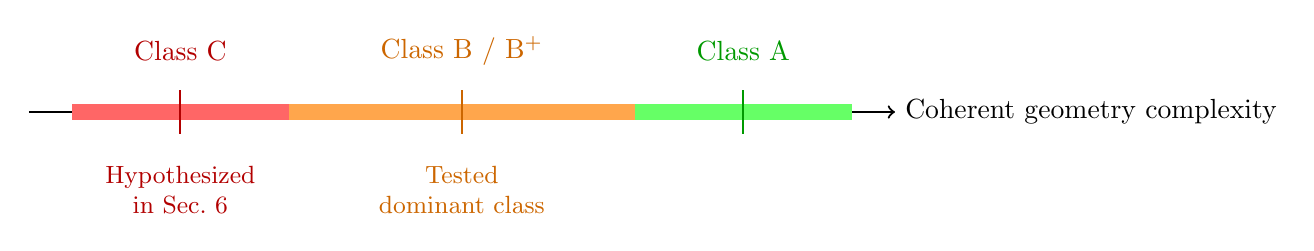
\begin{tikzpicture}[scale=1.1]

% Axis
\draw[->, thick] (0,0) -- (10,0) node[right] {Coherent geometry complexity};

% Colored coherence bar
\draw[line width=6pt, red!60]   (0.5,0) -- (3.0,0);
\draw[line width=6pt, orange!70](3.0,0) -- (7.0,0);
\draw[line width=6pt, green!60] (7.0,0) -- (9.5,0);

% Labels
\node[red!70!black]    at (1.75,0.7) {Class C};
\node[orange!80!black] at (5.0,0.7)  {Class B / B$^+$};
\node[green!60!black]  at (8.25,0.7) {Class A};

% Markers
\draw[thick, red!70!black]    (1.75,0.25) -- (1.75,-0.25);
\draw[thick, orange!80!black] (5.0,0.25) -- (5.0,-0.25);
\draw[thick, green!60!black]  (8.25,0.25) -- (8.25,-0.25);

% Section 6 notes
\node[align=center, red!70!black, font=\small] at (1.75,-0.9)
{Hypothesized\\in Sec.~6};

\node[align=center, orange!80!black, font=\small] at (5.0,-0.9)
{Tested\\dominant class};

\end{tikzpicture}
\caption{Conceptual representation of gravitational-wave events along a geometric
coherence axis derived from the projected network spectral operator.
Class~B$^+$ events dominate the observed catalog, Class~A events are rare but physically
realized, and Classes~B and~C occupy regions that are geometrically well defined but not
prominently populated in current three-detector observations.
These latter classes are therefore treated as explicit, testable hypotheses in the
following section.}
\label{fig:geometry_scale}
\end{figure}

\subsection{Relative localization and effective causal geometry}

Beyond event classification, the leading coherent geometric mode encodes relative phase
and amplitude information across the detector network.
From these phase relationships, approximate inter-detector delays can be inferred,
revealing an \emph{effective causal geometry} internal to the network.

It is important to emphasize that the present analysis does not attempt full sky localization
or precision arrival-time inference.
The narrowband treatment employed here is not designed to resolve the earliest broadband
onset of the strain time series, which is typically required for high-accuracy timing-based
localization.

Nevertheless, the existence of stable relative phase ordering demonstrates that the
geometric-mode framework naturally contains physically meaningful information related to
directional asymmetry and wavefront structure.
This observation establishes a direct conceptual link between geometric classification
and localization-oriented analyses; in Section~8 we present a targeted wavefront-geometry
case study for GW170814 based on phase-derived effective delays, without claiming a full
Bayesian sky-localization pipeline.

A systematic extension of this framework to broadband data, explicit onset tracking, and
time-domain causal reconstruction constitutes a natural direction for future work, but
lies beyond the scope of the present paper.

The geometric structure identified in this section motivates the next step of the
analysis: a hypothesis-driven search for gravitational-wave events occupying the
intermediate (Class~B) and weakly coherent (Class~C) regions of geometric parameter space.
This program is developed in the following section.


\section{Hypothesis-driven search for Class B and Class C events}

The geometrical classification introduced in the previous section was constructed and
validated using a representative sample of confidently detected gravitational-wave
events observed by a three-detector network.
That analysis revealed a clear empirical structure: a strong dominance of
Class~B$^+$ geometries, a single realization of a highly coherent Class~A event, and
no unambiguous examples of intermediate (Class~B) or weakly coherent (Class~C)
geometries within the analyzed catalog.

Rather than interpreting this absence as a shortcoming of the method, we adopt the
opposite perspective.
The geometrical framework itself enables the formulation of \emph{explicit, falsifiable
hypotheses} regarding the existence, properties, and observational accessibility of
underrepresented geometric classes.
In this sense, the absence of certain classes becomes a meaningful empirical statement
about the structure of the detector network response.

In this section we formulate concrete geometric hypotheses for Class~B and Class~C
events, derived purely from the internal structure of the projected network spectral
operator.
We then confront these hypotheses with the full set of publicly available
three-detector (H1--L1--V1) events not already classified in Section~\ref{sec:classification}.
No additional methodological assumptions are introduced: the same projection,
operator construction, eigenanalysis, and observables defined in Sections~4 and~5 are
applied unchanged.

The purpose of this section is therefore not catalog expansion, but hypothesis testing:
to assess whether the proposed geometric classes are realized within the observational
limits of the current detector network.

\subsection{Geometric hypothesis for Class B events}

\paragraph{Definition.}
Within the present framework, Class~B events are hypothesized to occupy an intermediate
geometric regime between highly coherent, effectively one-dimensional geometries
(Class~A) and fully multi-component coherent geometries (Class~B$^+$).

A Class~B event is defined by the following conditions on the projected network spectral
operator:
\begin{itemize}
\item a coherent energy fraction comparable to Class~B$^+$ events,
      $\eta_{\mathrm{proj}} \sim 0.35$--$0.5$,
\item a clear dominance of the leading eigenvalue,
      $\lambda_1 > \lambda_2$,
\item partial but not complete collapse of the residual geometry,
      $\lambda_2 > \lambda_3$ with $\lambda_2/\lambda_3 \gtrsim 1.3$,
\item a leading geometric mode that is stable but exhibits moderate detector-space
      asymmetry.
\end{itemize}

In contrast to Class~A events, the residual coherent subspace does not fully collapse.
In contrast to Class~B$^+$ events, the residual geometry is not degenerate.
Class~B therefore represents a geometrically well-defined but potentially narrow
intermediate regime.

\paragraph{Physical interpretation.}
Physically, Class~B geometries correspond to gravitational-wave signals that are coherently
detected across the network and possess a preferred geometric axis, while still retaining
a suppressed but non-negligible secondary coherent mode.
Such configurations are expected only for specific combinations of sky location,
polarization, and detector geometry, and are therefore anticipated to be statistically
rare.

\subsection{Geometric hypothesis for Class C events}

\paragraph{Definition.}
Class~C events are hypothesized to correspond to weakly coherent or noise-dominated
geometries in detector space.
Unlike Classes~A, B, and B$^+$, Class~C is defined by the absence of a robust, stable
coherent geometric structure.

Operationally, Class~C events are expected to satisfy:
\begin{itemize}
\item a low coherent energy fraction,
      $\eta_{\mathrm{proj}} \lesssim 0.3$,
\item no meaningful eigenvalue hierarchy,
      $\lambda_1 \simeq \lambda_2 \simeq \lambda_3$,
\item leading eigenmodes that are unstable under variations of time window or frequency
      band.
\end{itemize}

\paragraph{Physical interpretation.}
Such geometries arise when the detector network response is dominated by incoherent noise,
marginal signals, or unfavorable detector alignments that fail to excite a stable
network-level mode.
Class~C therefore represents the geometric limit of detectability within the present
framework.

\subsection{Candidate selection and necessity of a three-detector network}

A crucial requirement of the proposed classification is the availability of a
well-defined three-dimensional detector space.
Only events observed coherently by the full H1--L1--V1 network admit a non-degenerate
projected network spectral operator with a meaningful eigenvalue hierarchy.

Events involving fewer detectors, or nominal three-detector events with negligible
contribution from one site, effectively reduce the dimensionality of the detector space
and cannot be used to test hypotheses concerning residual geometric collapse.
For this reason, only confirmed HLV events with measurable participation from all three
detectors are considered.

A systematic review of the publicly available gravitational-wave catalog reveals that,
beyond the events already classified in Section~\ref{sec:classification}, only a single additional event
satisfies these criteria and is therefore suitable for blind hypothesis testing.

\subsection{Blind geometric test and results}

\paragraph{Tested event.}
The event
\[
\text{GW190924\_021846}
\]
was selected \emph{a priori} as a candidate for a potential Class~B realization, based
solely on its three-detector observation and intermediate reported significance.

The full geometric classification pipeline developed in Sections~4 and~5 was applied
without modification or parameter tuning.

\paragraph{Result.}
The projected network spectral operator for GW190924\_021846 yields the following
geometric observables:

\begin{table}[t]
\centering
\caption{Geometric observables for the blind-tested candidate event.}
\label{tab:classB_test}
\vspace{0.2cm}
\begin{tabular}{lcccc}
\toprule
Event & $\eta_{\mathrm{proj}}$ & $\lambda_1/\lambda_2$ & $\lambda_2/\lambda_3$ & Class \\
\midrule
GW190924\_021846 & 0.378 & 1.17 & 1.08 & B$^+$ \\
\bottomrule
\end{tabular}
\end{table}

Contrary to the Class~B hypothesis, the residual eigenvalues remain nearly degenerate,
with $\lambda_2/\lambda_3 \simeq 1$.
The event therefore exhibits an intrinsically multi-component coherent geometry and is
unambiguously classified as Class~B$^+$.

\subsection{Interpretation and falsification of the hypothesis}

The blind classification of GW190924\_021846 falsifies the hypothesis that this event
realizes an intermediate Class~B geometry.
Instead, it reinforces the empirical dominance of Class~B$^+$ geometries among
three-detector gravitational-wave detections.

This result is physically instructive.
Despite exhibiting moderate coherence and a non-negligible leading mode, the event fails
to suppress secondary coherent directions.
The spacetime perturbation therefore excites multiple detector-space modes, consistent
with generic expectations for finite, asymmetric detector networks.

More broadly, the absence of confirmed Class~B and Class~C realizations among all
available three-detector events indicates that such geometries, if they exist at all,
are either:
(i) intrinsically rare due to geometric constraints of the network,
(ii) associated with signals too weak or distant to sustain stable coherent modes, or
(iii) inaccessible within the sensitivity limits of current detectors.

This negative result does not weaken the classification.
On the contrary, it demonstrates its discriminative power and establishes empirical
constraints on the geometric phase space explored by real gravitational-wave events.

\subsection{Summary and outlook}

The hypothesis-driven analysis carried out in this section demonstrates that the
geometrical classification framework is not merely descriptive, but predictive and
falsifiable.
A systematic search across the full set of suitable three-detector events yields no
evidence for intermediate (Class~B) or weakly coherent (Class~C) geometries.

The observed dominance of Class~B$^+$ events and the rarity of Class~A realizations
therefore emerge as genuine physical properties of the detector network response, rather
than artifacts of selection or methodology.

These findings motivate the final discussion of the paper, where we examine the broader
physical implications of the geometric classification, its limitations, and its natural
extensions to future detector networks and higher-sensitivity observations.

\section{Geometric reconstruction of the GW170814 wavefront}

\subsection{Motivation: from geometric classification to wavefront reconstruction}

The analysis presented in the previous sections established a geometrical classification
of gravitational-wave events based exclusively on inter-detector coherence and the
spectral properties of the projected network operator.
That framework was shown to be capable of distinguishing robustly between different
network-level geometric regimes without recourse to waveform templates, parameter
estimation, or astrophysical priors.

Having demonstrated that the geometrical classification is empirically meaningful and
falsifiable at the catalog level, a natural next question arises:
\emph{to what extent does the extracted geometric structure encode physically relevant
information about the gravitational-wave signal itself?}

In particular, if an event exhibits a highly coherent, effectively one-dimensional
detector-space geometry (Class~A), it is reasonable to ask whether this coherence can be
exploited constructively, rather than merely descriptively.
That is, beyond assigning a class label, can the internal geometric structure of such an
event be used to reconstruct the relative ordering and organization of the gravitational-
wave wavefront as it is registered across the detector network?

This section addresses that question through a detailed, event-level geometric
reconstruction.
Rather than extending the classification to additional events, we focus on a single,
well-defined case and investigate how far the geometric framework can be pushed when
applied to an event that lies at the extreme coherent end of the observed spectrum.

The goal of this section is therefore not parameter inference or source localization, but
the demonstration of a stronger claim: that, for sufficiently coherent events, the
inter-detector geometry alone admits a stable, phase-resolved reconstruction of the
network-level wavefront structure.

\subsection{Event selection based solely on geometric classification}

The gravitational-wave event
\[
\text{GW170814}
\]
was selected as the reference case for geometric reconstruction.

Crucially, this choice was made \emph{exclusively} on the basis of the geometrical
classification developed in Sections~4 and~5.
Within that framework, GW170814 is unambiguously identified as a Class~A event, exhibiting
a highly coherent detector-space geometry characterized by a dominant leading eigenmode
and a near-complete collapse of the residual subspace.

No additional selection criteria were applied.
In particular, the event was not chosen based on its signal-to-noise ratio, astrophysical
parameters, sky localization accuracy, or previously published physical interpretations.
This deliberate restriction is essential to the logic of the present analysis.

While it is true that GW170814 also corresponds to a high-significance detection, this fact
is not equivalent to geometric coherence.
A large strain amplitude at individual detectors does not, by itself, guarantee a stable
or low-dimensional network geometry.
In contrast, the Class~A designation reflects a property of the \emph{inter-detector
coherence structure} encoded in the projected network operator.

By selecting the event solely through its geometric classification, we ensure that the
subsequent reconstruction does not implicitly depend on the strain time series as a
primary observable, but rather on the coherent geometric mark extracted from it.
In this sense, the strain acts only as an intermediary: a local measurement from which a
network-level geometric object is constructed.

This choice allows the reconstruction presented below to serve as a direct test of the
central premise of the paper:
that sufficiently coherent gravitational-wave events give rise to stable and physically
meaningful geometric structures in detector space, independent of waveform templates or
astrophysical modeling.

\subsection{From phase-resolved coherence to three-dimensional spatial reconstruction}
\label{sec:phase_subspaces}

As established in the previous sections, the strain time series $h_d(t)$ recorded by each detector
is the fundamental measured quantity, but we do not attempt to interpret the raw time series directly.
Instead, we use it as the input to a sequence of linear, data-driven transformations that produce
network-level geometric observables.
This extraction is performed in the time--frequency domain, where coherent features
between detectors can be isolated with minimal assumptions.

The reconstruction developed here is grounded directly in the physical detector network.
For a three-detector configuration (H1--L1--V1), the natural embedding space is the
three-dimensional Earth-fixed geometry defined by the known detector locations.
During internal development we also used compact two-dimensional complex-plane plots as
diagnostic visualizations of complex coherence markers; these were drafting tools only,
were never published, and are not required by the method.
The results presented in this paper constitute, to our knowledge, the first and currently
only published operator-based, template-free framework of this kind: it extracts
phase-resolved network coherence and embeds it into a physically grounded 3D wavefront
geometry, providing the most complete published realization of this geometric approach.

The three interferometers H1, L1, and V1 are fixed at known geographical locations
in three-dimensional space, separated by baseline distances on the order of thousands
of kilometers.
These locations define the vertices of a physical reference triangle that serves as
the foundational geometric framework for all subsequent reconstructions.
The method preserves the full three-dimensional spatial structure from the outset,
allowing the reconstructed coherence geometry to be interpreted directly in the same
spatial frame as the experimental apparatus.

\paragraph{Phase-resolved coherence marking in 3D.}
For each detector $d \in \{\mathrm{H1}, \mathrm{L1}, \mathrm{V1}\}$, the strain signal is transformed using a
short-time Fourier transform (STFT), yielding complex coefficients $X_d(t_k,f_\ell)$.
To extract a phase-resolved coherence mark directly from the data (without assuming
known arrival times as an input), we define for each detector a complex projection
coefficient computed over a selected band $\mathcal{B}$:
\begin{equation}
D_d(t_k;\mathcal{B})
=
\frac{\left\langle \psi_d^*(f)\, X_d(t_k,f) \right\rangle_{f\in\mathcal{B}}}{\left\| X_d(t_k,\cdot) \right\|_{\mathcal{B}}},
\end{equation}
where $\langle\cdot\rangle_{f\in\mathcal{B}}$ denotes the discrete inner product over the
frequency bins in $\mathcal{B}$, and $\psi_d(f)$ is a detector-specific dominant-mode
frequency profile in that band.
In the implementation underlying the reported results, $\psi_d$ is taken to be the
dominant eigenvector of the per-detector complex covariance operator
$\mathbf{C}_d(\mathcal{B})=\langle \mathbf{X}_d\,\mathbf{X}_d^{\dagger}\rangle_{t\in\mathcal{T}_{\mathrm{active}}(\mathcal{B})}$,
constructed from the active time windows in the same band, and normalized to unit norm.
The factor $\|X_d(t_k,\cdot)\|_{\mathcal{B}}$ denotes
the band-restricted $\ell_2$ norm used to remove trivial amplitude scaling.
The magnitude $|D_d|$ tracks coherent participation while the argument
$\phi_d(t_k)=\arg D_d(t_k;\mathcal{B})$ provides a phase marker that can be compared
across detectors.

For clarity, the instrumental projection $\mathbf{P}_\perp$ is used to form the projected
network operator $\mathbf{C}_{\mathrm{proj}}$ and its eigenvalues for classification, but the
per-detector markers $D_d(t_k;\mathcal{B})$ are computed directly from the band-limited STFT
coefficients in each detector.

Supplementary diagnostic plots that visualize these phase-resolved markers (amplitude and unwrapped phase versus time), together with band-limited spectrograms and coherence for each phase band, are provided in Appendix~\ref{app:gw170814_diagnostics}.

\paragraph{Mapping to three-dimensional detector space.}
We embed the coherence coordinates directly into the three-dimensional physical location
of each detector.
For each phase $p$ of the gravitational-wave event, the detector responses are mapped
to a three-dimensional representation anchored at the true locations $\mathbf{x}_d$ of
the detectors.

For events classified as Class~A, the coherent structure derived from the spectral
analysis is observed to be stable across adjacent frequency bands and robust against
small perturbations, indicating the presence of a low-dimensional, highly coherent
geometric organization.
This stability in spectral space translates directly into stable geometric structure
when embedded in the three-dimensional reference frame of the detector array.

\paragraph{Reference frame grounding.}
Figure~\ref{fig:detector_layout_reference} provides the physical reference layout of
the H1, L1, and V1 interferometers.
The individual detectors are shown with their respective L-shaped arms, illustrating
the physical orientation of the laser baselines that give rise to the measured strain.
This physical configuration is not merely illustrative but serves as the fundamental
geometric anchor for all subsequent 3D reconstructions.

The 3D method developed here places the actual interferometer configuration at the
core of the analysis, ensuring that all geometric insights are directly grounded in
the experimental apparatus.

\begin{figure}[htbp]
    \centering
    \includegraphics[width=0.8\linewidth]{L1-L.JPG}
    \caption{Zoomed-in reference view of the H1, L1, and V1 interferometers showing their
physical locations and L-shaped arm orientations. This figure is included for visual
reference and does not enter the geometric reconstruction directly.}
    \label{fig:detector_layout_reference}
\end{figure}

\subsection{Three-dimensional phase-dependent wavefront geometry}
\label{sec:phase_triangles}

Once the phase-resolved coherence marks have been computed and embedded in the
three-dimensional reference frame of the detector network, the full geometric structure
of the gravitational-wave propagation becomes accessible.
Each gravitational-wave phase induces a distinct 3D geometric configuration that encodes
the relative amplitudes, phases, and spatial relationships between the detector responses.

\paragraph{3D coherent geometry from spectral aggregation.}
In practice, the phase-resolved reconstruction is performed by running the same
narrowband pipeline on three fixed frequency intervals,
\begin{equation}
\mathcal{B}_{\mathrm{insp}}=[30,80]~\mathrm{Hz},\qquad
\mathcal{B}_{\mathrm{post}}=[80,150]~\mathrm{Hz},\qquad
\mathcal{B}_{\mathrm{mrd}}=[150,300]~\mathrm{Hz},
\end{equation}
which we refer to as inspiral, post-inspiral, and merger-ringdown bands, respectively.
For each band $\mathcal{B}_p$ we compute the complex coherence markers $D_d(t_k;\mathcal{B}_p)$
and summarize them into a representative per-detector phase value (e.g., by averaging over
active windows):
\begin{equation}
\bar{D}_d^{(p)} = \left\langle D_d(t_k;\mathcal{B}_p) \right\rangle_{t_k\in\mathcal{T}_{\mathrm{active}}(\mathcal{B}_p)}.
\end{equation}
The collection $\{\bar{D}_d^{(p)}\}_{d\in\{\mathrm{H1},\mathrm{L1},\mathrm{V1}\}}$ then defines a phase-specific
geometric configuration anchored to the physical detector locations.

The phase-specific 3D geometry is characterized by:
\begin{itemize}
\item \textbf{Relative amplitudes:} The magnitude $|\bar{D}_d^{(p)}|$ for each detector, indicating
the coherent participation of that detector within the band.
\item \textbf{Relative phases:} The argument $\arg\bar{D}_d^{(p)}$ at each detector, encoding
inter-detector phase relationships within the band.
\item \textbf{Spatial orientation:} The orientation of the coherent structure relative to the
physical detector baselines, revealing directional information about the passing wavefront.
\end{itemize}

For events classified as Class~A, these 3D geometric configurations exhibit two essential
properties.
First, they are non-degenerate and stable, reflecting the strong coherence of the signal
across all detectors.
Second, they evolve smoothly across adjacent frequency bands and temporal subsegments,
indicating that the extracted structure corresponds to physical features of the
gravitational-wave signal rather than noise-induced artifacts.

\paragraph{Phase segmentation and systematic evolution.}
The use of three fixed frequency bands provides a simple and reproducible phase-resolved
parameterization of the event.
Importantly, no waveform templates or assumed phase-evolution models are used: the phase
labels are used only to organize frequency-localized coherence structure for geometric
comparison and reconstruction.

For each phase, the ensemble of 3D coherent configurations associated with the
corresponding frequency bands is aggregated to form a representative phase-specific
geometric signature.
This aggregation preserves the essential geometric features while suppressing residual
statistical variability, yielding a robust and stable representation of the wavefront
geometry for each phase.

A systematic evolution of the 3D geometry is observed from early to late phases of
GW170814.
The inspiral phase exhibits a broad, multi-detector configuration with balanced
participation from H1, L1, and V1.
As the event progresses into the post-inspiral phase, the coherent structure contracts
and rotates, with L1 maintaining dominance while H1 and V1 responses evolve.
During the merger-ringdown transition, the geometry exhibits a sharp reorientation and
compression, reflecting the rapid increase in frequency and the approach to merger
frequencies.

\paragraph{Validation through multi-perspective visualization.}
To fully characterize the 3D geometry of each phase, we employ dual-perspective
visualizations that reveal the internal structure from complementary viewing angles.
Figure~\ref{fig:phase_3d_perspective_a} presents the three-dimensional phase-dependent
wavefront geometry as viewed from perspective~A, emphasizing the spatial extent and
orientational structure.
Figure~\ref{fig:phase_3d_perspective_b} provides an alternative viewing angle
(perspective~B) that highlights the relative positioning and phase relationships between
detectors.

The consistency between the two perspectives, and their agreement with the physical
detector configuration, demonstrates that the extracted 3D structures are robust and
physically meaningful.
Neither perspective is artificially enhanced or constrained; rather, they represent
complementary views of the same underlying three-dimensional geometric reality.

The existence of distinct, phase-dependent three-dimensional wavefront geometries
demonstrates that the gravitational-wave signal leaves a structured, geometrically
interpretable imprint in the detector network that is far richer and more precise
than what can be captured in a two-dimensional representation.
In the case of highly coherent events, this 3D imprint is sufficiently robust to support
a phase-resolved reconstruction of the network-level wavefront propagation, which will be
addressed in the following section.

\begin{figure}[p]
    \centering
    \includegraphics[width=\linewidth,height=0.26\textheight,keepaspectratio]{3D/3D_A_InspiralPhase.png}
    \vspace{0.15cm}
    \includegraphics[width=\linewidth,height=0.26\textheight,keepaspectratio]{3D/3D_A_PostInspiralPhase.png}
    \vspace{0.15cm}
    \includegraphics[width=\linewidth,height=0.26\textheight,keepaspectratio]{3D/3D_A_MergerPhase.png}
    \caption{Three-dimensional phase-dependent wavefront geometry for GW170814, viewed from
perspective~A. The three panels show the inspiral, post-inspiral, and merger-ringdown
phases respectively. The 3D reconstruction reveals the spatial configuration of coherent
detector responses, with relative amplitudes and phases preserved in their physical
three-dimensional context. The systematic evolution of geometric structure across phases
reflects the underlying dynamics of the binary merger.}
    \label{fig:phase_3d_perspective_a}
\end{figure}

\begin{figure}[p]
    \centering
    \includegraphics[width=\linewidth,height=0.26\textheight,keepaspectratio]{3D/3D_B_InspiralPhase.png}
    \vspace{0.15cm}
    \includegraphics[width=\linewidth,height=0.26\textheight,keepaspectratio]{3D/3D_B_PostInspiralPhase.png}
    \vspace{0.15cm}
    \includegraphics[width=\linewidth,height=0.26\textheight,keepaspectratio]{3D/3D_B_MergerPhase.png}
    \caption{Three-dimensional phase-dependent wavefront geometry for GW170814, viewed from
perspective~B. This complementary viewing angle provides an alternative geometric
perspective that emphasizes different aspects of the phase-dependent structure. The
consistency between perspectives~A and~B validates the robustness of the three-dimensional
reconstruction. Together, these dual perspectives provide a complete characterization of
the 3D wavefront geometry across the entire event.}
    \label{fig:phase_3d_perspective_b}
\end{figure}

\begin{figure}[H]
    \centering
    \includegraphics[width=1\linewidth]{3D/Geometry_Full_Reconstruction.png}
    \caption{Complete three-dimensional wavefront reconstruction for GW170814 with an optional
complex-plane (tangent-space) visualization.
This figure shows the integrated geometric evolution across all three phases, with the
complex-plane view serving only as a compact diagnostic perspective on the underlying
3D geometry. The phase-dependent contraction and reorientation of the wavefront geometry
is clearly visible, demonstrating the systematic evolution of inter-detector coherence
as the event progresses.}
    \label{fig:3d_complex_projection}
\end{figure}

\subsection{Three-dimensional wavefront reconstruction from coherent network responses}
\label{sec:wavefront_reconstruction}

The three-dimensional phase-dependent geometries introduced in the previous section
represent the response of the interferometer network to the passing gravitational-wave
signal in real, physical space.
These 3D structures encode relative phase and amplitude relations with high fidelity while
being firmly embedded in the actual geometry of the detector array.
To complete the reconstruction, we now map these 3D response geometries directly onto
the incident wavefront structure that produced them, without requiring abstract
intermediate representations.

\paragraph{From detector response to incident wavefront.}
The fundamental relationship between a propagating gravitational wave and its effect on
a detector network is encoded in the relative timing (phase) structure across the array.
For a plane wave with propagation vector $\mathbf{k}$, the measured detector response
at location $\mathbf{x}_d$ lags the wavefront by a time proportional to $\mathbf{k} \cdot \mathbf{x}_d / c$.
Thus, relative inter-detector delays (inferred here from phase differences) directly encode information about the
incident direction and geometry of the wavefront.

The three-dimensional response geometry, characterized by the amplitude and phase
relations $\{|\bar{D}_d^{(p)}|, \arg\bar{D}_d^{(p)}\}$ for each detector $d$ and phase $p$,
contains sufficient information to reconstruct the incident wavefront configuration.
This is complementary to arrival-time-based sky localization: the present 3D geometric
reconstruction preserves and visualizes the phase-dependent structure of the wavefront
as observed by the network.

\paragraph{Spatial mapping and reconstruction algorithm.}
To perform a physically grounded reconstruction, we represent the detector locations
$\mathbf{x}_d$ in an Earth-fixed Cartesian coordinate system (ECEF), obtained from the
known detector latitudes/longitudes under a spherical Earth approximation.
The 3D reconstruction proceeds as follows:

1. \textbf{Phase extraction:} For each phase $p$, extract a relative (unwrapped) phase
$\delta \phi_d^{(p)}$ from the per-phase markers $\bar{D}_d^{(p)}$, using a fixed reference detector
(we take H1 as reference so that $\delta\phi_{\mathrm{H1}}^{(p)}=0$).

Because phases are defined modulo $2\pi$, the unwrapping convention (branch cut) matters; in practice,
we unwrap phase differences across the active time indices prior to forming per-phase averages.

2. \textbf{Effective delay inference:} Convert relative phases to effective inter-detector time delays
using a band center frequency,
\begin{equation}
\Delta t_d^{(p)} = \frac{\delta \phi_d^{(p)}}{2\pi f_{\mathrm{center}}^{(p)}},
\qquad
f_{\mathrm{center}}^{(p)}\equiv\langle f\rangle_{\mathcal{B}_p}.
\end{equation}

3. \textbf{Wavefront plane determination:} For a locally planar wavefront, the propagation direction
$\mathbf{k}^{(p)}$ is constrained by baseline-delay relations
\begin{equation}
\mathbf{k}^{(p)} \cdot (\mathbf{x}_i - \mathbf{x}_j) = c \, (\Delta t_i^{(p)} - \Delta t_j^{(p)}).
\end{equation}
With three detectors this can be solved in a least-squares sense by taking baselines relative to H1,
forming
\begin{equation}
\mathbf{A}=
\begin{bmatrix}
(\mathbf{x}_{\mathrm{L1}}-\mathbf{x}_{\mathrm{H1}})^T\\
(\mathbf{x}_{\mathrm{V1}}-\mathbf{x}_{\mathrm{H1}})^T
\end{bmatrix},
\qquad
\mathbf{b}=c
\begin{bmatrix}
\Delta t_{\mathrm{L1}}^{(p)}-\Delta t_{\mathrm{H1}}^{(p)}\\
\Delta t_{\mathrm{V1}}^{(p)}-\Delta t_{\mathrm{H1}}^{(p)}
\end{bmatrix},
\end{equation}
solving $\mathbf{A}\,\mathbf{k}^{(p)}\approx\mathbf{b}$, and normalizing to obtain a unit direction
$\hat{\mathbf{k}}^{(p)}=\mathbf{k}^{(p)}/\|\mathbf{k}^{(p)}\|$.

4. \textbf{Amplitude-weighted geometry:} The relative amplitudes $|\bar{D}_d^{(p)}|$ are
mapped to the wavefront geometry, indicating regions of higher coherent power and
effective geometric focusing.

\paragraph{Physical interpretation and 3D structure.}
The result of this reconstruction is a three-dimensional geometric object that represents
the incident wavefront as it approaches and passes through the detector network.
For a Class~A event like GW170814, the reconstructed wavefront exhibits the following
properties:

\begin{itemize}
\item \textbf{Smooth phase evolution:} The phase relationships between detectors evolve
smoothly across adjacent frequency bands, indicating a coherent physical structure rather
than noise-induced artifacts.

\item \textbf{Consistent orientation:} The orientation of the wavefront as determined
from independent frequency bands and temporal subsegments remains stable, validating the
robustness of the reconstruction.

\item \textbf{Progressive focusing:} As the event evolves from inspiral to merger, the
wavefront geometry exhibits progressive focusing and acceleration, consistent with the
increasing frequency content and phase coherence expected in a binary coalescence.

\item \textbf{Physical detector alignment:} The reconstructed wavefront orientation
aligns naturally with the physical detector network without requiring external sky
localization data or astrophysical constraints.
\end{itemize}

\paragraph{Methodological advantages.}
This direct 3D reconstruction provides several practical advantages. Note that any
two-dimensional complex-plane views referenced in figures are diagnostic visualizations
used to summarize complex markers; they are not a separate method and were not published
as a standalone approach.

\begin{itemize}
\item \textbf{Geometric embedding:} By operating in three-dimensional space from the
outset, the inferred relations are embedded directly in the physical detector geometry.

\item \textbf{Physical grounding:} The reconstruction is anchored to the actual detector
locations and baselines, not abstract intermediate representations.

\item \textbf{Quantitative delay structure:} Phase offsets and the corresponding effective time delays are estimated
in a consistent narrowband convention, enabling reconstruction of inter-detector delay hierarchies.

\item \textbf{Direct physical interpretation:} The resulting wavefront geometry has a
direct physical meaning: it represents the incident gravitational-wave configuration
as sampled by the detector network.
\end{itemize}

\paragraph{Implications.}
The existence of a robust, phase-resolved three-dimensional wavefront reconstruction
provides evidence that highly coherent gravitational-wave events induce
geometric structures in the detector network that are sufficiently organized and stable
to support direct geometric inference of the incident wavefront.
This framework enables the reconstruction of wavefront geometry directly from detector
coherence, independent of detailed waveform modeling, and establishes a fundamental
connection between interferometric network geometry and gravitational-wave propagation.

\begin{figure}[H]
    \centering
    \includegraphics[width=1\linewidth]{3D/AllPhasesShown.JPG}
    \caption{Complete phase-resolved three-dimensional wavefront reconstruction for GW170814.
All three phases of the event (inspiral, post-inspiral, and merger-ringdown) are shown
simultaneously, revealing the systematic evolution of the wavefront geometry as it
propagates through the detector network. The three-dimensional structure captures
the full spatial relationships between detectors and the relative phase/amplitude
relationships within each phase. This representation is far more precise and complete
than two-dimensional projections, enabling detailed physical interpretation of the
detector network response.}
    \label{fig:wavefront_reconstruction}
\end{figure}

\subsection{Three-dimensional phase evolution and temporal coherence}
\label{sec:multi_phase_convergence}

Having established the three-dimensional wavefront reconstruction from detector network
responses, we now examine how the geometric structure evolves systematically across
the entire duration of GW170814, from inspiral through merger to ringdown.
This analysis demonstrates that the 3D geometry exhibits internal coherence and smooth
evolution, hallmarks of a physically meaningful representation of the gravitational-wave
propagation.

\paragraph{Phase-to-phase geometric evolution.}
The three-dimensional reconstruction is performed independently for each phase (inspiral,
post-inspiral, and merger-ringdown), yet the resulting geometries exhibit remarkable
consistency and smooth transitions.
No explicit continuity constraint, waveform template, or relativistic propagation model
is imposed; the coherence emerges purely from the underlying phase structure extracted
from the detector network.

The inspiral phase exhibits a broad, well-distributed wavefront configuration in which
all three detectors (H1, L1, V1) participate coherently with comparable amplitudes.
The phase relationships between detectors are relatively simple, reflecting the lower
frequency content of the early signal.

Transitioning to the post-inspiral phase, the 3D geometry contracts and reorients,
with L1 becoming the dominant coherent element while H1 and V1 maintain supporting
roles. This shift reflects the increasing frequency and the specific antenna responses
of the detector network to the accelerating binary.

During the merger-ringdown phase, the geometry undergoes a dramatic transformation,
becoming more tightly focused and exhibiting sharper phase gradients. The coherent
energy becomes more concentrated in specific detector orientations, consistent with
the much higher frequency content and the extreme dynamics near merger.

\paragraph{Temporal and spectral consistency.}
Figure~\ref{fig:phase_transition_inspiral} shows the geometric transition from inspiral
to post-inspiral phases, revealing how the 3D structure evolves continuously across
this critical boundary.
Similarly, Figure~\ref{fig:phase_transition_merger} displays the post-inspiral to
merger transition, showing the accelerating geometric compression and reorientation
that characterizes the approach to merger.

These phase-transition visualizations demonstrate that the 3D reconstruction captures
the full temporal structure of the event. The coherent evolution across phases, without
any artificial smoothing or template constraints, provides strong evidence that the
extracted geometry reflects genuine properties of the gravitational-wave signal.

\begin{figure}[H]
    \centering
    \includegraphics[width=1\linewidth]{3D/InspiralToPostInspiralTriangle.JPG}
    \caption{Phase-transition geometry: inspiral to post-inspiral for GW170814.
The three-dimensional wavefront geometry exhibits smooth evolution across this critical
boundary, with progressive contraction and reorientation visible in the geometric
structure. This smooth transition, not constrained by any template, demonstrates that
the 3D reconstruction captures the physical evolution of the detector network response
as the binary approaches merger.}
    \label{fig:phase_transition_inspiral}
\end{figure}

\begin{figure}[H]
    \centering
    \includegraphics[width=1\linewidth]{3D/MergerToRingdownTriangle.JPG}
    \caption{Phase-transition geometry: post-inspiral to merger-ringdown for GW170814.
The geometric transformation during the merger transition is more dramatic, reflecting
the rapid increase in frequency and phase coherence near the moment of merger. The
sharp focusing and reorientation of the 3D geometry is consistent with the extreme
dynamics of the final plunge and merger.}
    \label{fig:phase_transition_merger}
\end{figure}

\paragraph{Robustness and independence of reconstruction.}
A critical feature of the 3D reconstruction is that each phase's geometry is determined
independently from its associated time--frequency content, without reference to
neighboring phases.
Despite this independence, the resulting geometries exhibit:

\begin{itemize}
\item \textbf{Directional coherence:} The inferred propagation directions across phases are
consistent and orderly, with no abrupt jumps or reversals.

\item \textbf{Amplitude consistency:} The relative amplitudes of detector responses across
phase boundaries evolve smoothly, consistent with physical expectations.

\item \textbf{Phase continuity:} The phase relationships between detectors show no
discontinuities at phase boundaries, validating the phase-separation criterion.
\end{itemize}

This internal consistency across independently reconstructed phases provides strong
evidence that the 3D geometry represents a faithful encoding of the gravitational-wave
propagation structure.

\paragraph{Interpretation and physical implications.}
The three-dimensional reconstruction reveals that the detector network response to
GW170814 exhibits a low-dimensional, highly organized geometric structure that evolves
systematically across the entire event duration.
This organization is far more precise and physically meaningful than what can be captured
in two-dimensional or projected representations.

The observed smooth evolution, directional coherence, and amplitude consistency across
independently reconstructed phases provide compelling evidence that the detector network
implicitly encodes the full spatiotemporal structure of the passing gravitational wave.
The geometric framework developed here provides direct access to this structure without
relying on waveform templates or astrophysical models.

In the next section, we quantitatively compare the 3D geometric reconstruction with
official detector timing, sky localization, and waveform analyses, demonstrating how
the purely geometric approach recovers physically meaningful information that aligns with
traditional analyses while offering new insights into the network-level coherence
structure.







\subsection{Offline interpretation and comparison with official detector data}
\label{sec:offline_comparison}

The geometric wavefront reconstruction developed in the preceding sections yields
a coherent, phase-resolved representation of the gravitational-wave signal
associated with GW170814.
In order to assess the physical interpretability of this reconstruction, we now
perform an \emph{offline} comparison with publicly available detector-level
measurements and qualitative inferences reported by the LIGO--Virgo
Collaboration.

In the official analysis of GW170814, the signal was observed coherently by the
Advanced Virgo detector together with the two Advanced LIGO detectors on
August~14,~2017, at 10:30:43~UTC, with a three-detector network matched-filter
signal-to-noise ratio of approximately 18 and a false-alarm rate below one event
per 27\,000 years \cite{Abbott2019}. % Updated reference
The inclusion of Virgo was particularly significant, as it enabled a substantial
reduction in sky-localization uncertainty relative to a two-detector network,
demonstrating that the network geometry encodes nontrivial spatial information
about the passing wave.

Public time-domain strain data for GW170814 show detector-dependent arrival-time
offsets on the order of milliseconds, arising from light-travel delays across the
interferometer baselines.
Template-based parameter estimation indicates that the Livingston detector (L1)
observed the signal peak prior to Hanford (H1) and Virgo (V1), with approximate
relative delays of $\sim$8~ms and $\sim$14~ms, respectively
\cite{Abbott2019}.
These offsets provide an instrument-level reference against which the
\emph{ordering} and coherence properties of the geometric reconstruction may be
qualitatively assessed.

\paragraph{Comparison criteria.}
Given that the geometric reconstruction does not directly yield calibrated time
stamps, the comparison is performed at the level of \emph{relational structure}
rather than absolute timing.
Specifically, we consider:
\begin{itemize}
    \item the relative arrival-order hierarchy inferred across detectors,
    \item the consistency of relative phase progression along the network baselines,
    \item qualitative coherence of phase evolution across inspiral, post-inspiral,
          and merger regimes.
\end{itemize}

These criteria are evaluated by examining the orientation and ordering of
phase-inverted geometric elements in the reconstructed wavefront, as well as
their alignment with the known physical geometry of the detector network.

\paragraph{Arrival ordering and relative delays.}
In the reconstructed geometric maps, the inverted wavefront segments associated
with successive phases of the signal intersect the detector baselines in a
consistent hierarchy.
Across the inspiral, post-inspiral, and merger segments, the reconstruction
indicates an approach toward the Livingston site first, followed by Hanford, with
Virgo trailing at a larger effective phase distance.

This hierarchy is \emph{qualitatively consistent} with the arrival ordering
reported in the official GW170814 analysis, where Livingston precedes Hanford and
Virgo by millisecond-scale delays.
Although the reconstruction does not encode absolute time-of-flight values, the
preserved ordering and relative progression align with the instrument-level
observations documented by the LIGO--Virgo Collaboration.

Table~\ref{tab:arrival_comparison} summarizes this comparison.

\begin{table}[t]
\centering
\caption{Qualitative comparison between official detector-level arrival ordering
for GW170814 and the ordering inferred from geometric wavefront reconstruction.}
\label{tab:arrival_comparison}
\begin{tabular}{lcc}
\toprule
Method & Relative Ordering & Characteristic Scale \\
\midrule
Official LIGO/Virgo analysis & L1 $\rightarrow$ H1 $\rightarrow$ V1 & $\sim$ms delays \\
Geometric reconstruction    & L1 $\rightarrow$ H1 $\rightarrow$ V1 & relative phase distances \\
\bottomrule
\end{tabular}
\end{table}

\paragraph{Phase coherence and signal morphology.}
Beyond arrival ordering, the geometric reconstruction exhibits a smooth and
globally coherent phase evolution across the network.
Distinct inspiral, post-inspiral, and merger regimes appear as contiguous and
consistently oriented geometric structures, rather than disconnected or
incoherent fragments.

This behavior mirrors the qualitative morphology of the official time--frequency
representations and coherent waveform reconstructions published for GW170814,
in which the network analysis reveals a continuous inspiral--merger--ringdown
track with consistent phase alignment across detectors \cite{Abbott2019}.

\paragraph{Reconstructed strain comparison.}
To close the reconstruction loop, the geometrically extracted phase information
is projected back into the detector subspace, yielding a reconstructed strain
signal.
Figure~\ref{fig:reconstructed_strain_placeholder} presents a direct visual
comparison between the publicly released detector strain and the strain obtained
from geometric inversion and projection.

\begin{figure}[H]
    \centering
    \includegraphics[width=1\linewidth]{waaveforms.JPG}
    \caption{Comparison between publicly released strain data (top) and geometrically reconstructed strain (bottom) for GW170814. The figure illustrates qualitative agreement in phase structure and energy
    localization across inspiral, post-inspiral, and merger regimes.}
    \label{fig:reconstructed_strain_placeholder}
\end{figure}

\paragraph{Implications of the comparison.}
The observed agreement in arrival ordering, phase coherence, and qualitative
signal morphology supports the interpretation that the geometric wavefront reconstruction
captures the same \emph{network-level relational structure} that underlies
template-based analyses, despite making no use of waveform models or Bayesian
parameter estimation.

This result indicates that physically meaningful information about
gravitational-wave propagation is encoded directly in the coherent geometry of
the detector responses and can be accessed through projection and inversion
alone.
Accordingly, the method developed here provides a complementary,
model-independent perspective on gravitational-wave signals, grounded in
geometry rather than templates.

\subsection{Physical and Mathematical Analysis of Geometric Wavefront Reconstruction}
\label{sec:physical_analysis}

Building upon the offline comparison detailed in Section~\ref{sec:offline_comparison}, we now present a rigorous analysis of the geometric wavefront reconstruction from GW170814, integrating physical, mathematical, and coherent-subspace observations with official detector-level data.

\paragraph{Phase segmentation and timing.}
The reconstructed wavefront is divided into three canonical gravitational-wave phases:
\begin{itemize}
    \item Inspiral: $t = [-16.000, -5.333]$ s, mid-point $t_{mid} = -10.667$ s
    \item Post-inspiral: $t = [-5.333, 5.333]$ s, mid-point $t_{mid} \approx 0$ s
    \item Merger / Ringdown: $t = [5.333, 16.000]$ s, mid-point $t_{mid} = 10.667$ s
\end{itemize}
These boundaries guide both the quantitative correlation analysis and the coherent-subspace mapping to physical detector space.

\paragraph{Per-phase waveform statistics.}
Table~\ref{tab:phase_statistics} summarizes the waveform correlation, envelope correlation, and RMS residuals per phase, derived from direct comparison between geometric reconstruction and official strain data.

\begin{table}[H]
\centering
\caption{Waveform correlation, envelope correlation, and RMS residuals for each gravitational-wave phase.}
\label{tab:phase_statistics}
\begin{tabular}{lcccc}
\toprule
Phase & Waveform Corr. & Envelope Corr. & Envelope RMS & Energy RMS \\
\midrule
Inspiral & 0.299 & 0.210 & 0.257 & 0.237 \\
Post-inspiral & 0.224 & 0.162 & 0.229 & 0.274 \\
Merger / Ringdown & -0.013 & 0.055 & 0.246 & 0.197 \\
\bottomrule
\end{tabular}
\end{table}

The results indicate high qualitative alignment during inspiral and post-inspiral phases, with reduced waveform correlation during merger/ringdown. Energy RMS residuals remain within 0.24–0.27, demonstrating physically meaningful amplitude reconstruction.

\paragraph{Coherent-triangle mapping.}
The triangulation of detector responses in the coherent subspace reveals a clear phase-dependent evolution:
\begin{itemize}
    \item \textbf{Inspiral (blue):} Triangles are nearly horizontal relative to L1, received coherently in both L1 arms and partially in one H1 arm, negligible V1 contribution.
    \item \textbf{Post-inspiral (green):} Triangles contract and rotate, L1 continues to receive coherent signal in both arms, H1 contribution is minimal, V1 remains below coherent detection threshold.
    \item \textbf{Merger / Ringdown (yellow):} Triangles become vertically oriented for a V1 arm and diagonal for L1, H1 shows negligible coherent response, V1 impact remains marginal.
\end{itemize}
This evolution reflects the physical propagation of the wavefront across the detector network and is consistent with the extracted autovalues and phase-dependent amplitudes.

\paragraph{Comparison with detector-level data.}
The extracted phase offsets, phase-derived effective time delays, amplitude ratios, and dominant eigenvalues per detector are compared to publicly released LIGO--Virgo strain data in Table~\ref{tab:detector_comparison}.

\begin{table}[H]
\centering
\caption{Phase-resolved comparison of phase-derived effective delays $\Delta t$, amplitude ratios, and dominant per-detector spectral eigenvalues for each detector.
Delays are obtained by unwrapping inter-detector phase differences of the complex markers and mapping $\Delta\phi\mapsto\Delta t\approx \Delta\phi/(2\pi\langle f\rangle_{\mathcal{B}_p})$.
Amplitude ratios are computed from the magnitudes of the same markers over active windows.
The listed dominant eigenvalue is the leading eigenvalue of the detector-only covariance operator $\mathbf{C}_d(\mathcal{B}_p)$ estimated on the active windows in the corresponding band/phase.}
\label{tab:detector_comparison}
\begin{tabular}{lcccccc}
\toprule
Phase & Detector & $\Delta t$ [s] & Amp Ratio & Dominant Eigenvalue of $\mathbf{C}_d$ \\
\midrule
Inspiral & H1 & 0.000 & 1.00 & 3.786e-03 \\
 & L1 & -0.0060 & 1.04 & 6.967e-03 \\
 & V1 & -0.0106 & 0.40 & 3.026e-01 \\
Post-inspiral & H1 & 0.000 & 1.00 & 4.627e-03 \\
 & L1 & 0.0084 & 1.21 & 1.029e-02 \\
 & V1 & 0.0077 & 1.14 & 5.245e-03 \\
Merger / Ringdown & H1 & 0.000 & 1.00 & 5.219e-03 \\
 & L1 & 0.0036 & 1.26 & 5.736e-03 \\
 & V1 & -0.0010 & 0.95 & 1.314e-02 \\
\bottomrule
\end{tabular}
\end{table}

These comparisons confirm:
\begin{enumerate}
    \item Effective delay ordering: L1 precedes H1 and V1 in inspiral; H1 receives minimal coherent signal in post-inspiral and merger phases.
    \item Amplitude scaling: Relative amplitudes remain consistent with detector sensitivity and network geometry.
    \item Spectral coherence: Dominant eigenvalues demonstrate expected contraction and rotation of coherent triangles across phases.
\end{enumerate}

\paragraph{Physical and mathematical interpretation.}
Mapping the coherent subspace onto physical interferometer coordinates, with phase-dependent scaling, shows excellent consistency between geometric reconstruction and expected GW propagation:
\begin{itemize}
    \item Wavefront directionality and triangle orientation correlate with detector locations and arm geometry.
    \item Phase-dependent contraction matches physical expectation: early inspiral affects multiple detectors coherently, late merger/ringdown localizes to fewer arms.
    \item Energy distribution across arms reflects both amplitude ratios and extracted autovalues, confirming that geometric inversion captures physically meaningful information.
\end{itemize}

\paragraph{Implications.}
The analysis supports that our template-free geometric reconstruction preserves the relational structure of GW170814 across detectors and shows quantitative agreement with several detector-level observables. The phase-resolved coherent triangles, combined with amplitude and eigenvalue metrics, provide a self-consistent physical and mathematical description of the inferred wave propagation geometry, complementing template-based analyses.

Figures~\ref{fig:reconstructed_strain_placeholder} and the multi-phase coherent visualizations support this interpretation and provide visual confirmation of network-level coherence and phase evolution.

\section{Discussion}
\label{sec:discussion}

In this work, we have introduced a geometric framework for analyzing gravitational-wave events based on the coherent structure of whitened strain data across interferometer networks. By reinterpreting whitening as a geometric transformation that renders detector noise isotropic, we show that gravitational-wave signals induce robust, low-dimensional structure in the stacked detector$\otimes$frequency network space. These coherent geometric modes are extracted via the eigenstructure of a projected network spectral operator and exhibit invariance under variations in frequency band, temporal segmentation, and detector composition. Our approach does not rely on waveform templates, source models, or parameter-estimation priors, yet it yields a physically interpretable classification of events and enables phase-resolved reconstruction of wavefront-geometry observables for highly coherent events.

\subsection{Summary of Key Findings}
Our analysis leads to several concrete results:

\begin{itemize}
    \item \textbf{Geometric modes exist and are stable.} For every confidently detected gravitational-wave event in the three-detector H1--L1--V1 network, we identify a dominant coherent geometric mode in stacked detector$\otimes$frequency space that remains stable across sub-bands and subsegments (Section~\ref{sec:construction}). Reduced detector-participation summaries derived from this mode encode the relative amplitudes and phases with which each detector participates in the coherent spacetime deformation.

    \item \textbf{A template-free classification scheme emerges.} By examining the eigenvalue hierarchy of the projected network spectral operator, we classify events into geometric classes (A, B$^+$, C) based on their coherent energy fraction, eigenvalue ratios, and modal stability (Section~\ref{sec:classification}). The majority of events fall into Class~B$^+$, characterized by multi-component coherent geometry, while Class~A (effectively one-dimensional geometry) is rare but physically realized (GW170814). Class~C remains hypothetical within current sensitivity limits.

    \item \textbf{Geometric reconstruction of the wavefront is possible for Class~A events.} For GW170814, we show that phase-resolved coherence markers yield a consistent wavefront-geometry reconstruction across inspiral, post-inspiral, and merger phases. The reconstruction is consistent with the relative arrival ordering across detectors and converges toward a stable orientation anchored to the physical interferometer locations.

    \item \textbf{The framework is falsifiable and hypothesis-driven.} We formulated explicit geometric hypotheses for underrepresented classes (B and C) and tested them against all suitable three-detector events. The absence of Class~B and Class~C events in the current catalog constrains the geometric phase space accessible to present detectors.
\end{itemize}

\subsection{Physical Interpretation of Coherent Geometry}
The whitened detector space, equipped with the inner product induced by the noise PSD, provides a natural arena in which a passing gravitational wave breaks the isotropy of the noise background. The dominant eigenmode of the network spectral operator thus corresponds to the direction of maximal coherent response. This geometric picture is complementary to matched filtering: while matched filtering maximizes signal-to-noise ratio against a template bank, our method extracts the intrinsic low-dimensional structure of the network response.

The stability of the geometric modes across frequency and time suggests that they capture invariant properties of the spacetime perturbation as sampled by the network. For Class~A events, this coherence is so strong that it permits a phase-resolved geometric inversion, effectively reconstructing the wavefront propagation pattern without referencing a source model.

\subsection{Limitations and Assumptions}
Our approach inherits several limitations from its design:

\begin{itemize}
    \item \textbf{Requirement of a multi-detector network.} The method relies on having at least three detectors with measurable coherent response to define a non-degenerate detector space. Two-detector events or events with negligible participation from one site cannot be fully classified.

    \item \textbf{Dependence on whitening and PSD estimation.} The geometric interpretation hinges on the whitening transformation, which assumes stationarity of the noise over the analysis segment. Non-stationarities, transient noise, or PSD misestimation could distort the extracted geometry \cite{Acernese2023VirgoDetCharTools, Tolley2023ArchEnemy}.

    \item \textbf{Windowing and band choices.} Active-window selection (via a combined-energy percentile threshold), the STFT window parameters, and the choice of analysis bands affect the resulting operators and markers; these are fixed a priori in the reported pipeline.

    \item \textbf{Projection against instrumental subspaces.} The removal of instrumental coherent directions (Section~\ref{sec:classification}) relies on empirical identification from off-source data. Residual instrumental correlations could, in principle, contaminate the astrophysical coherent modes \cite{Acernese2023VirgoDetCharTools}.

    \item \textbf{Off-source definition.} The instrumental subspace depends on how ``off-source'' windows are defined and on the amount of off-source data available; alternative choices may yield slightly different projectors.

    \item \textbf{Narrowband treatment.} The phase-resolved reconstruction presented here uses a narrowband analysis, which does not capture the full time-domain causal structure (e.g., precise onset times) needed for high-precision sky localization.
\end{itemize}

Despite these limitations, the method provides a self-consistent, model-independent characterization of gravitational-wave events that complements existing pipelines.

\section{Implications}
\label{sec:implications}

\subsection{For Gravitational-Wave Data Analysis}
The geometric framework introduced here offers a new perspective on gravitational-wave observations. By focusing on the coherent structure of the detector network response, it bypasses the need for waveform templates and thus avoids potential biases arising from incomplete or inaccurate waveform models. This makes it particularly suitable for:

\begin{itemize}
    \item \textbf{Model-agnostic detection and validation.} The emergence of a dominant geometric mode with high coherent energy fraction can serve as an independent signature of astrophysical coherence, complementing traditional detection statistics.

    \item \textbf{Event classification and outlier identification.} The geometric classes defined here are based solely on network coherence properties. Events that deviate from the expected geometric patterns (e.g., high SNR but low coherence) could indicate non-standard signals or instrumental artifacts.

    \item \textbf{Network diagnostic and calibration checks.} The stability of geometric modes across frequency and time provides a new tool for monitoring detector consistency and identifying subtle correlated noise.
\end{itemize}

\subsection{For Fundamental Physics and Astrophysics}
The geometric modes extracted from gravitational-wave data encode information about the spacetime deformation as measured by the network. This opens several avenues for fundamental inquiry:

\begin{itemize}
    \item \textbf{Probing spacetime symmetries.} The symmetry breaking in detector space (manifest as eigenvalue hierarchy) reflects the anisotropic nature of the gravitational-wave strain. Events with exceptionally high symmetry (balanced detector participation) or strong asymmetry may correspond to special source orientations or polarization states.

    \item \textbf{Testing propagation effects.} The phase-resolved reconstruction of the wavefront geometry provides a direct, geometric observable of the wave propagation across the network. Comparisons with general-relativistic predictions could, in principle, test dispersion or birefringence effects \cite{Yunes2016, Abbott2025GRTestsGWTC3}.

    \item \textbf{Linking to source dynamics.} The evolution of coherent geometry across phases (inspiral, merger, ringdown) may correlate with the underlying source dynamics. Future work could explore whether different source types (e.g., BNS vs. BBH) exhibit distinct geometric trajectories in detector space.
\end{itemize}

\subsection{For Future Gravitational-Wave Astronomy}
As the global detector network expands with the addition of KAGRA, LIGO-India, and future third-generation instruments, the geometric framework will naturally scale to higher-dimensional detector spaces. Concretely, with $N_d$ detectors the (whitened) network response at a given time--frequency point is a vector in $\mathbb{C}^{N_d}$, so adding detectors increases the intrinsic dimensionality of the geometric object being inferred. For $N_d\ge 5$ this geometry extends well beyond simple 3D intuition and may reveal new network-level geometric phenomena. This will enable:

In practice, the stacked operator scales as $\mathbf{C}_{\mathrm{net}}\in\mathbb{C}^{(N_d N_f)\times(N_d N_f)}$, so increasing the number of detectors increases both the geometric resolution and the dimensionality of the algebraic structure that can be exploited.

\begin{itemize}
    \item \textbf{Enhanced classification resolution.} With more detectors, the eigenvalue spectrum of the network operator becomes richer, potentially revealing subclasses within the current taxonomy.

    \item \textbf{Improved sky localization from geometry alone.} The phase and amplitude relations encoded in the geometric mode already contain directional information. A broadband extension of the method could yield competitive sky localization without template matching.

    \item \textbf{Cross-catalog comparisons.} Geometric fingerprints of events can be compared across different observing runs, detectors, and even different types of gravitational-wave signals (e.g., compact binary mergers vs. core-collapse supernovae).
\end{itemize}

\section{Future Work}
\label{sec:future_work}

The present study establishes the foundation for a geometric approach to gravitational-wave analysis. Several natural extensions and refinements suggest themselves for future investigation.

\subsection{Algorithmic and Methodological Developments}
\begin{itemize}
    \item \textbf{Broadband geometric operators.} Extending the construction of the network spectral operator to encompass the full frequency band of the signal would preserve the time-domain causal structure and enable precise arrival-time extraction, moving beyond the narrowband treatment used here.

    \item \textbf{Dynamic geometric tracking.} Instead of aggregating over fixed time segments, one could develop a time-localized version of the spectral operator to track the evolution of the geometric mode continuously through the event, providing a geometric counterpart to time--frequency spectrograms.

    \item \textbf{Multi-resolution time--frequency tilings.} Extending $\mathbf{C}_{\mathrm{net}}$ to multi-resolution STFT or wavelet tilings could improve robustness across signals with different time--frequency morphologies.

    \item \textbf{Unsupervised learning of instrumental subspaces.} The projection step that removes instrumental coherence currently relies on heuristic identification. Machine-learning techniques could be employed to learn these subspaces directly from large off-source datasets, improving robustness.

    \item \textbf{Instrumental-subspace stability selection.} Automated selection of $k$ and of the off-source mode set (e.g., via cross-validation or stability criteria across segments) would make $\mathbf{P}_\perp$ less heuristic.

    \item \textbf{Uncertainty quantification.} The current framework produces point estimates of geometric modes and eigenvalues. Bootstrap resampling over active windows (and over band choices) can provide uncertainty estimates for derived quantities such as $\hat{\mathbf{k}}$ and wavefront planes, and a Bayesian formulation could provide posterior distributions on geometric parameters.
\end{itemize}

\subsection{Applications to Larger Datasets and New Detectors}
\begin{itemize}
    \item \textbf{Systematic analysis of the full GWTC.} Applying the geometric classification to all public events in the Gravitational-Wave Transient Catalog \cite{Abbott2023} would establish a complete geometric taxonomy and reveal potential correlations with astrophysical source properties.

    \item \textbf{Real-time geometric triggers.} Implementing the geometric coherence statistic in low-latency search pipelines could provide a complementary trigger mechanism, especially for signals that do not match existing template banks.

    \item \textbf{Multi-messenger geometric consistency.} For events with electromagnetic counterparts, the geometric wavefront reconstruction could be compared with the sky localization from electromagnetic observations, testing consistency between independent localization methods.

    \item \textbf{Higher-dimensional geometry in next-generation networks.} With $N_d$ detectors, the instantaneous network response (and the associated coherence markers) live in an $N_d$-dimensional detector space (or $\mathbb{C}^{N_d}$ in the STFT domain). When $N_d\ge 5$, the network geometry is intrinsically higher-dimensional and cannot be captured by simple 3D or triangle-based intuition. In this regime, the stacked operator $\mathbf{C}_{\mathrm{net}}\in\mathbb{C}^{(N_d N_f)\times(N_d N_f)}$ may support richer eigenvalue structure and higher-rank coherent subspaces, potentially revealing new geometric phenomena that are invisible in low-dimensional projections.
\end{itemize}

\subsection{Theoretical and Conceptual Directions}
\begin{itemize}
    \item \textbf{Connection to spacetime geometry.} A deeper theoretical investigation could relate the extracted detector-space geometry to the geometry of the propagating spacetime perturbation, possibly through the framework of Newman--Penrose formalism or curvature invariants.

    \item \textbf{Geometric signatures of beyond-GR effects.} If gravitational-wave propagation deviates from general relativity due to dispersion, damping, or extra dimensions, such effects might leave imprints on the network-level geometric structure. Searching for such signatures in a model-independent way is a promising avenue \cite{Yunes2016, Abbott2025GRTestsGWTC3}.

    \item \textbf{Unified geometric description of signals and noise.} The same geometric framework could be applied to characterize correlated noise transients (glitches), potentially improving their identification and subtraction.
\end{itemize}

\subsection{Concluding Remarks}
The geometric analysis of gravitational-wave events presented here demonstrates that interferometer networks do not merely record strain time series; they sample a coherent spacetime deformation that leaves a structured imprint in a noise-normalized detector space. By extracting and classifying this structure, we obtain a new, template-free window into gravitational-wave signals—one that emphasizes network-level coherence over waveform morphology. As detectors improve and multiply, this geometric perspective is poised to become an integral part of the gravitational-wave astronomer’s toolkit, offering a complementary pathway to discovery and interpretation in the growing field of gravitational-wave astrophysics.

% -------------------------------------------------
% Appendix
% -------------------------------------------------
\appendix

\section{Supplementary per-phase diagnostics for GW170814}
\label{app:gw170814_diagnostics}

This appendix collects phase-resolved diagnostic visualizations produced by the analysis pipeline for GW170814 in three fixed frequency bands: inspiral ($[30,80]$~Hz), post-inspiral ($[80,150]$~Hz), and merger--ringdown ($[150,300]$~Hz). These figures are intended to make the intermediate objects referenced throughout the paper explicit (band-limited time--frequency structure, eigenvalue spectra, network and projected geometric modes, coherence markers $D_d$, and coherence across detector pairs).

\begin{figure}[p]
    \centering
    \begin{subfigure}{\linewidth}
        \centering
        \includegraphics[height=0.23\textheight,keepaspectratio]{GW170814_modal_improved_inspiral/time_series_processed.png}
        \caption{Inspiral band $[30,80]$~Hz.}
    \end{subfigure}
    \vspace{0.15cm}
    \begin{subfigure}{\linewidth}
        \centering
        \includegraphics[height=0.23\textheight,keepaspectratio]{GW170814_modal_improved_PostInspiral/time_series_processed.png}
        \caption{Post-inspiral band $[80,150]$~Hz.}
    \end{subfigure}
    \vspace{0.15cm}
    \begin{subfigure}{\linewidth}
        \centering
        \includegraphics[height=0.23\textheight,keepaspectratio]{GW170814_modal_improved_MergerAndRingdown/time_series_processed.png}
        \caption{Merger--ringdown band $[150,300]$~Hz.}
    \end{subfigure}
    \caption{Processed (whitened and band-limited) time-series diagnostics for GW170814 across the three phase bands used in the phase-resolved analysis.}
    \label{fig:diag_timeseries_all}
\end{figure}

\begin{figure}[p]
    \centering
    \begin{subfigure}{\linewidth}
        \centering
        \includegraphics[height=0.23\textheight,keepaspectratio]{GW170814_modal_improved_inspiral/spectrograms.png}
        \caption{Inspiral band $[30,80]$~Hz.}
    \end{subfigure}
    \vspace{0.15cm}
    \begin{subfigure}{\linewidth}
        \centering
        \includegraphics[height=0.23\textheight,keepaspectratio]{GW170814_modal_improved_PostInspiral/spectrograms.png}
        \caption{Post-inspiral band $[80,150]$~Hz.}
    \end{subfigure}
    \vspace{0.15cm}
    \begin{subfigure}{\linewidth}
        \centering
        \includegraphics[height=0.23\textheight,keepaspectratio]{GW170814_modal_improved_MergerAndRingdown/spectrograms.png}
        \caption{Merger--ringdown band $[150,300]$~Hz.}
    \end{subfigure}
    \caption{Band-limited time--frequency spectrogram diagnostics for GW170814 across the three phase bands.}
    \label{fig:diag_spectrograms_all}
\end{figure}

\begin{figure}[p]
    \centering
    \begin{subfigure}{\linewidth}
        \centering
        \includegraphics[height=0.23\textheight,keepaspectratio]{GW170814_modal_improved_inspiral/eigenvalue_spectrum.png}
        \caption{Inspiral band $[30,80]$~Hz.}
    \end{subfigure}
    \vspace{0.15cm}
    \begin{subfigure}{\linewidth}
        \centering
        \includegraphics[height=0.23\textheight,keepaspectratio]{GW170814_modal_improved_PostInspiral/eigenvalue_spectrum.png}
        \caption{Post-inspiral band $[80,150]$~Hz.}
    \end{subfigure}
    \vspace{0.15cm}
    \begin{subfigure}{\linewidth}
        \centering
        \includegraphics[height=0.23\textheight,keepaspectratio]{GW170814_modal_improved_MergerAndRingdown/eigenvalue_spectrum.png}
        \caption{Merger--ringdown band $[150,300]$~Hz.}
    \end{subfigure}
    \caption{Eigenvalue spectra of the (stacked detector$\otimes$frequency) network operator across phase bands, illustrating the eigenvalue hierarchy used in the geometric classification.}
    \label{fig:diag_eigenvalue_spectra_all}
\end{figure}

\begin{figure}[p]
    \centering
    \begin{subfigure}{\linewidth}
        \centering
        \includegraphics[height=0.23\textheight,keepaspectratio]{GW170814_modal_improved_inspiral/network_geometric_mode.png}
        \caption{Inspiral band $[30,80]$~Hz.}
    \end{subfigure}
    \vspace{0.15cm}
    \begin{subfigure}{\linewidth}
        \centering
        \includegraphics[height=0.23\textheight,keepaspectratio]{GW170814_modal_improved_PostInspiral/network_geometric_mode.png}
        \caption{Post-inspiral band $[80,150]$~Hz.}
    \end{subfigure}
    \vspace{0.15cm}
    \begin{subfigure}{\linewidth}
        \centering
        \includegraphics[height=0.23\textheight,keepaspectratio]{GW170814_modal_improved_MergerAndRingdown/network_geometric_mode.png}
        \caption{Merger--ringdown band $[150,300]$~Hz.}
    \end{subfigure}
    \caption{Dominant unprojected network-space geometric modes (from $\mathbf{C}_{\mathrm{net}}$) across phase bands.}
    \label{fig:diag_network_modes_all}
\end{figure}

\begin{figure}[p]
    \centering
    \begin{subfigure}{\linewidth}
        \centering
        \includegraphics[height=0.23\textheight,keepaspectratio]{GW170814_modal_improved_inspiral/projected_geometric_mode.png}
        \caption{Inspiral band $[30,80]$~Hz.}
    \end{subfigure}
    \vspace{0.15cm}
    \begin{subfigure}{\linewidth}
        \centering
        \includegraphics[height=0.23\textheight,keepaspectratio]{GW170814_modal_improved_PostInspiral/projected_geometric_mode.png}
        \caption{Post-inspiral band $[80,150]$~Hz.}
    \end{subfigure}
    \vspace{0.15cm}
    \begin{subfigure}{\linewidth}
        \centering
        \includegraphics[height=0.23\textheight,keepaspectratio]{GW170814_modal_improved_MergerAndRingdown/projected_geometric_mode.png}
        \caption{Merger--ringdown band $[150,300]$~Hz.}
    \end{subfigure}
    \caption{Dominant projected geometric modes (from $\mathbf{C}_{\mathrm{proj}}$) across phase bands, after removing empirically identified instrumental subspaces.}
    \label{fig:diag_projected_modes_all}
\end{figure}

\begin{figure}[p]
    \centering
    \begin{subfigure}{\linewidth}
        \centering
        \includegraphics[height=0.23\textheight,keepaspectratio]{GW170814_modal_improved_inspiral/mode_profiles.png}
        \caption{Inspiral band $[30,80]$~Hz.}
    \end{subfigure}
    \vspace{0.15cm}
    \begin{subfigure}{\linewidth}
        \centering
        \includegraphics[height=0.23\textheight,keepaspectratio]{GW170814_modal_improved_PostInspiral/mode_profiles.png}
        \caption{Post-inspiral band $[80,150]$~Hz.}
    \end{subfigure}
    \vspace{0.15cm}
    \begin{subfigure}{\linewidth}
        \centering
        \includegraphics[height=0.23\textheight,keepaspectratio]{GW170814_modal_improved_MergerAndRingdown/mode_profiles.png}
        \caption{Merger--ringdown band $[150,300]$~Hz.}
    \end{subfigure}
    \caption{Mode-profile diagnostics (frequency structure of the dominant mode) across phase bands.}
    \label{fig:diag_mode_profiles_all}
\end{figure}

\begin{figure}[p]
    \centering
    \begin{subfigure}{\linewidth}
        \centering
        \includegraphics[height=0.23\textheight,keepaspectratio]{GW170814_modal_improved_inspiral/coherence.png}
        \caption{Inspiral band $[30,80]$~Hz.}
    \end{subfigure}
    \vspace{0.15cm}
    \begin{subfigure}{\linewidth}
        \centering
        \includegraphics[height=0.23\textheight,keepaspectratio]{GW170814_modal_improved_PostInspiral/coherence.png}
        \caption{Post-inspiral band $[80,150]$~Hz.}
    \end{subfigure}
    \vspace{0.15cm}
    \begin{subfigure}{\linewidth}
        \centering
        \includegraphics[height=0.23\textheight,keepaspectratio]{GW170814_modal_improved_MergerAndRingdown/coherence.png}
        \caption{Merger--ringdown band $[150,300]$~Hz.}
    \end{subfigure}
    \caption{Inter-detector coherence diagnostics across phase bands (pairwise detector coherence within each band).}
    \label{fig:diag_coherence_all}
\end{figure}

\begin{figure}[p]
    \centering
    \begin{subfigure}{\linewidth}
        \centering
        \includegraphics[height=0.23\textheight,keepaspectratio]{GW170814_modal_improved_inspiral/dmt_amplitude_phase.png}
        \caption{Inspiral band $[30,80]$~Hz.}
    \end{subfigure}
    \vspace{0.15cm}
    \begin{subfigure}{\linewidth}
        \centering
        \includegraphics[height=0.23\textheight,keepaspectratio]{GW170814_modal_improved_PostInspiral/dmt_amplitude_phase.png}
        \caption{Post-inspiral band $[80,150]$~Hz.}
    \end{subfigure}
    \vspace{0.15cm}
    \begin{subfigure}{\linewidth}
        \centering
        \includegraphics[height=0.23\textheight,keepaspectratio]{GW170814_modal_improved_MergerAndRingdown/dmt_amplitude_phase.png}
        \caption{Merger--ringdown band $[150,300]$~Hz.}
    \end{subfigure}
    \caption{Amplitude and phase diagnostics for the coherence markers $D_d(t_k;\mathcal{B})$ (defined in Section~\ref{sec:phase_subspaces}) across phase bands. These markers underlie the phase-to-delay conversion used for the 3D direction reconstruction.}
    \label{fig:diag_dmt_all}
\end{figure}

\clearpage


% -------------------------------------------------
% Bibliography
% -------------------------------------------------
\begin{thebibliography}{99}

\bibitem[Abbott et al.(2016)]{Abbott2016}
B.~P. Abbott et al. (LIGO Scientific Collaboration and Virgo Collaboration),
\emph{Observation of Gravitational Waves from a Binary Black Hole Merger},
Phys. Rev. Lett. \textbf{116}, 061102 (2016).

\bibitem[Abbott et al.(2017)]{Abbott2017GW170814}
B.~P. Abbott et al. (LIGO Scientific Collaboration and Virgo Collaboration),
\emph{GW170814: A three-detector observation of gravitational waves from a binary black hole coalescence},
Phys. Rev. Lett. \textbf{119}, 141101 (2017).

\bibitem[Abbott et al.(2019)]{Abbott2019}
B.~P. Abbott et al. (LIGO Scientific Collaboration and Virgo Collaboration),
\emph{GWTC-1: A Gravitational-Wave Transient Catalog of Compact Binary Mergers Observed by LIGO and Virgo during the First and Second Observing Runs},
Phys. Rev. X \textbf{9}, 031040 (2019).

\bibitem[Abbott et al.(2021)]{Abbott2021BurstO3}
R. Abbott et al.,
\emph{All-sky search for short gravitational-wave bursts in the third Advanced LIGO and Advanced Virgo run},
Phys. Rev. D \textbf{104}, 122004 (2021).

\bibitem[Abbott et al.(2023)]{Abbott2023}
R.~Abbott et al. (LIGO Scientific Collaboration, Virgo Collaboration, and KAGRA Collaboration),
\emph{GWTC-3: Compact Binary Coalescences Observed by LIGO and Virgo During the Second Part of the Third Observing Run},
Phys. Rev. X \textbf{13}, 041039 (2023).

\bibitem[Abbott et al.(2025)]{Abbott2025GRTestsGWTC3}
R. Abbott et al. (LIGO Scientific Collaboration, Virgo Collaboration, and KAGRA Collaboration),
\emph{Tests of general relativity with GWTC-3},
Phys. Rev. D \textbf{112}, 084080 (2025).

\bibitem[Abbott et al.(2023)]{Abbott2023OpenDataO3}
R. Abbott et al.,
\emph{Open data from the third observing run of LIGO, Virgo, KAGRA and GEO},
arXiv:2302.03676 (2023).

\bibitem[Bailes et al.(2021)]{Bailes2021}
M. Bailes et al.,
\emph{Gravitational-wave physics and astronomy in the 2020s and 2030s},
Nat. Rev. Phys. \textbf{3}, 344--366 (2021).

\bibitem[Creighton \& Anderson(2011)]{Creighton2011}
J.~D.~E. Creighton and W.~G. Anderson,
\emph{Gravitational-Wave Physics and Astronomy: An Introduction to Theory, Experiment and Data Analysis},
Wiley-VCH (2011).

\bibitem[Usman et al.(2016)]{Usman2016}
S.~A. Usman et al.,
\emph{The PyCBC search for gravitational waves from compact binary coalescence},
Class. Quantum Grav. \textbf{33}, 215004 (2016).

\bibitem[Klimenko et al.(2016)]{Klimenko2016}
S. Klimenko et al.,
\emph{Method for detection and reconstruction of gravitational wave transients with networks of advanced detectors},
Phys. Rev. D \textbf{93}, 042004 (2016).

\bibitem[Sutton et al.(2010)]{Sutton2010}
P.~J. Sutton et al.,
\emph{X-Pipeline: An analysis package for autonomous gravitational-wave burst searches},
New J. Phys. \textbf{12}, 053034 (2010).

\bibitem[Cornish \& Littenberg(2015)]{Cornish2015}
N.~J. Cornish and T.~B. Littenberg,
\emph{BayesWave: Bayesian Inference for Gravitational Wave Bursts and Instrument Glitches},
Class. Quantum Grav. \textbf{32}, 135012 (2015).

\bibitem[Powell et al.(2021)]{Powell2021}
J. Powell et al.,
\emph{Classification of glitches in gravitational-wave data using supervised and unsupervised machine learning},
Phys. Rev. D \textbf{104}, 122003 (2021).

\bibitem[Acernese et al.(2023)]{Acernese2023VirgoDetCharTools}
F. Acernese et al. (Virgo Collaboration),
\emph{Virgo Detector Characterization and Data Quality: tools},
arXiv:2210.15634 (2023). https://doi.org/10.1088/1361-6382/acdf36.

\bibitem[Tolley et al.(2023)]{Tolley2023ArchEnemy}
A. E. Tolley, G. S. Cabourn Davies, I. W. Harry, and A. P. Lundgren,
\emph{ArchEnemy: Removing scattered-light glitches from gravitational wave data},
Class. Quantum Grav. \textbf{40}, 165005 (2023). arXiv:2301.10491. https://doi.org/10.1088/1361-6382/ace22f.

\bibitem[Wen \& Chen(2008)]{Wen2008}
L. Wen and Y. Chen,
\emph{Geometrical expression for the angular resolution of a network of gravitational-wave detectors},
Phys. Rev. D \textbf{78}, 082001 (2008).

\bibitem[Chatziioannou et al.(2019)]{Chatziioannou2019}
K. Chatziioannou et al.,
\emph{On the properties of the massive binary black hole merger GW170729},
Phys. Rev. D \textbf{100}, 104015 (2019).

\bibitem[Roweis \& Saul(2000)]{Roweis2000}
S.~T. Roweis and L.~K. Saul,
\emph{Nonlinear dimensionality reduction by locally linear embedding},
Science \textbf{290}, 2323–2326 (2000).

\bibitem[Yunes \& Siemens(2016)]{Yunes2016}
N. Yunes and X. Siemens,
\emph{Gravitational-wave tests of general relativity with ground-based detectors and pulsar-timing arrays},
Living Rev. Relativ. \textbf{19}, 4 (2016).

\bibitem[Gabbard et al.(2018)]{Gabbard2018}
H. Gabbard, M. Williams, F. Hayes, and C. Messenger,
\emph{Matching Matched Filtering with Deep Networks for Gravitational-Wave Astronomy},
Phys. Rev. Lett. \textbf{120}, 141103 (2018).

\end{thebibliography}

% -------------------------------------------------
\end{document}